\documentclass[]{usiinfthesis}
\usepackage{lipsum}
\usepackage[draft]{fixme}
\usepackage{tikz}
\usepackage{algorithm}
\usepackage[noend]{algpseudocode}
\usetikzlibrary{automata}
% \usepackage{adjustbox}
%\setstretch{1.05}

\usepackage{listings}

\newcommand{\aseeker}{{AccelSeeker}} 
\newcommand{\rseeker}{{RegionSeeker}} 
\newcommand{\multi}{MuLTiVersioning}
\newcommand{\simulator}{\texttt{gem5-aladdin}} 
\newcommand{\HW}{{Hardware}}
\newcommand{\SW}{{Software}}
\newcommand{\HLS}{{High Level Synthesis}}
\newcommand{\SoC}{{System-on-Chip}}
\newcommand{\htsf}{{H.264}}
\newcommand{\SoTA}{{state-of-the-art}}
\newcommand{\plm}{{private local memory}}
\newcommand{\plms}{{private local memories}}

\newcommand{\ML}{{Machine Learning}}
\newcommand{\RF}{{Random Forest}}
\newcommand{\SVM}{{Support Vector Machines}}
\newcommand{\NN}{{Near Neighbor}}
\newcommand{\ItRef}{{Iterative Refinement}}

\newcommand{\dataflow}{data flow}
\newcommand{\controlflow}{control flow}
\newcommand{\CFG}{Control Flow Graph}
\newcommand{\CFGs}{Control Flow Graphs}

\newcommand{\compute}{\texttt{compute bound}} 
\newcommand{\iobound}{\texttt{I/O bound}} 

%algorithms
\newcommand{\exact}{\textsf{exact}}
\newcommand{\greedy}{\textsf{greedy}}
\newcommand{\exactC}{\textsf{exact-on-cropped}}

% \newcommand{\htsf}{\texttt{h264}}
\newcommand{\adpcm}{\texttt{adpcm}}
\newcommand{\sha}{\texttt{sha}}
\newcommand{\jpeg}{\texttt{jpeg}}
\newcommand{\mpeg}{\texttt{mpeg2}}
\newcommand{\aes}{\texttt{aes}}
\newcommand{\dfmul}{\texttt{dfmul}}
\newcommand{\dfsin}{\texttt{dfsin}}
\newcommand{\gsm}{\texttt{gsm}}
\newcommand{\stencil}{\texttt{stencil}}

%change 'sl' to 'bf' for bold, or 'normalfont' for no special
%formatting
\captionsetup{labelfont={sl,sf}}

\lstdefinelanguage{algebra}
{morekeywords={import,sort,constructors,observers,transformers,axioms,if,
else,end},
sensitive=false,
morecomment=[l]{//s},
}


\title{Software Analysis for\\ Heterogeneous Computing Architectures} %compulsory
\subtitle{A research automation framework 
towards more efficient\\ HW/SW co-design} %optional 
\author{Georgios Zacharopoulos} %compulsory
\advisor{Professor Laura Pozzi} %compulsory
%\coadvisor{Co-Advisor} %optional
\Day{21} %compulsory
\Month{October} %compulsory
\Year{2019} %compulsory, put only the year
\place{Lugano} %compulsory
\programDirector{The PhD program Director \emph{pro tempore}} %compulsory


\committee{%
  \committeeMember{Alonzo Church}{University of California, Los Angeles, USA}
  \committeeMember{Alan M. Turing}{Princeton University, USA}
  %there can as many members as you like
} %the committee is compulsory

\dedication{To my parents Areti and Dimitris.\\For always being there for me.} %optional
\openepigraph{Legacy. What is a legacy?\\ Planting seeds in a garden you never get to see.}{Alexander Hamilton}
\openepigraph
{Men give me credit for some genius. All the genius I have lies in this; when I have a subject in hand, I study 
it profoundly. Day and night it is before me. My mind becomes pervaded with it. Then the effort that I have made 
is what people are pleased to call the fruit of genius. It is the fruit of labor and thought.} {Alexander Hamilton} %optional

\makeindex %optional, also comment out \theindex at the end

\begin{document}

\maketitle %generates the titlepage, this is FIXED

\frontmatter %generates the frontmatter, this is FIXED

\begin{abstract}
\textbf{NOTE: The abstract will be written in the end of the thesis.}\\
Performance increase, in terms of faster execution and higher energy efficiency, 
is a never-ending research endeavor  %story 
and does not come for free.
The breakdown of Dennard scaling, along with the seemingly inevitable end of 
Moore's law economic aspect, present a new challenge to computer architects striving to achieve
better performance in the modern computer systems. Heterogeneous computing is 
emerging as one of the solutions to overcome these limitations in order to keep the performance 
trend rising. This is achieved by turning the focus to specialized Hardware (HW) that 
can accelerate the execution of a Software (SW) application or a part of that application.
The goal is to design efficient HW/SW computer architectures, where a general purpose CPU
is coupled with a number of specialized HW accelerators.\\
The choice of which parts of an application to be accelerated, though, as well as the type 
of accelerators to be used, while taking into account the underlying memory system, are all
non-trivial research questions and depend heavily on the SW applications characteristics that
are going to be accelerated. Therefore, an in-depth SW analysis can be crucial, prior to 
designing a heterogeneous system, as it can provide valuable information and subsequently 
highly benefit performance. My initial research is revolving around various ways that SW
analysis, by extending the compiler frameworks and, hence, their potential, can offer this 
type of information and move one step closer towards optimizing and automating the design of hybrid HW/SW systems.
\end{abstract}

% \begin{abstract}[Zusammenfassung]
% optional, use only if  external advisor requires it in his/er
% language 
% \\

% \lipsum
% \end{abstract}

\begin{acknowledgements}
This is where I acknowledge people.

% \lipsum 
\end{acknowledgements}

\tableofcontents 
%\listoffigures %optional
% \listoftables %optional

\mainmatter

%
%
%  
%     INTRO
%
%
%

\chapter*{Introduction}
\addcontentsline{toc}{chapter}{Introduction}

Performance increase, in terms of faster execution and higher energy efficiency, 
is a never-ending research domain and does not come for free.
Living in an era where there is an immense amount of data, the demand for %the execution
performance by modern computing systems rises even more.
Technological giants, such as Google and Facebook, gather and compute a lot of data, for instance 
during Machine Learning related applications and lengthy simulations. This large amount of data
processing requires a lot of computational power and ends up in lengthier and lengthier execution
latency time.\par

Moore's law \cite{schaller1997moore}, an observation made by the co-founder of Intel Gordon Moore, 
predicts that the number of transistors that can be used in the same area of an integrated 
circuit will double roughly every 18 months. Complimentary to that, Dennard scaling 
\cite{dennard1974design}, 
also known as MOSFET scaling, states that voltage and current are 
proportional to the size of a transistor. Therefore, as long as the same chip area is retained, 
power stays constant and, at the same time, more transistors of smaller size can fit onto it.
Unfortunately, this is no longer the case. The transistor size has decreased over 
the years, but the amount of power per transistor has, recently, stopped decreasing accordingly,  
resulting in current leakage, a phenomenon also known as the 
Breakdown of Dennard scaling \cite{esmaeilzadeh2011dark}.\par

The breakdown of Dennard scaling \cite{esmaeilzadeh2011dark}, along with the seemingly inevitable 
end of Moore's law economic aspect \cite{simonite2016moore}, present a new challenge to computer 
architects striving to achieve
better performance in the modern computer systems.
Heterogeneous computing is emerging as one of the solutions in order to keep the performance 
trend rising. This is achieved by turning the focus to specialized Hardware (HW) that 
can accelerate the execution of a Software (SW) application or a part of that application. Specialized HW 
accelerators are implemented in platforms where they can be either reprogrammable, 
thus allowing for a large degree of flexibility as various implementations may take place utilizing
the HW resources of the platform (e.g. an FPGA board), or hardwired, such as an Application-Specific Integrated 
Circuit (ASIC). The first type of HW implementations sacrifice part of the potential 
performance achieved by allowing for flexible designs, as the same HW resources can be reprogrammed.
The latter offer no flexibility but can provide better performance in comparison to FPGAs. Under 
the scope of this research both HW implementations were considered.  \par
%
% This is a link
%
Since the performance of a general purpose CPU is becoming limited, due to physical and technological 
constrains, alternative computer architectures are required. Homogeneous parallel CPUs are used in 
order to expose parallelism of computation in SW applications, but performance is still restricted 
by the parts of computation that cannot be parallelized, a fact known also as Amdahl's law.
Instead of a 
general purpose CPU -- or homogeneous parallel CPUs -- managing the execution of SW applications, 
specialized pieces
of HW, namely accelerators, can be used alongside with a general purpose CPU and execute the
most demanding parts of an application in terms of computation. Consequently, the need for 
a powerful single CPU is no more that critical, as the execution can be offloaded to other
parts of HW as well. %The gain is twofold, as 
As a result, we both achieve a more balanced execution with 
the use of different HW resources, and we offload the execution of specific, more demanding 
parts of the computation to specialized HW accelerators.\par
One example of a widely spread 
heterogeneous architecture is the addition of a GPU to a CPU on the same chip, in order 
to exploit the
parallelism and computing power that a GPU has to offer, when it comes to image processing 
and 3D graphics rendering. Other examples are general purpose CPUs coupled with dedicated HW
that execute specific kernels or even full applications. The latter architecture could come 
in a number of variations, with one or more HW accelerators, and different types of coupling, 
tightly or loosely \cite{CotaJun15}. The design of the first option, tightly or co-processor model, 
is done by using the accelerator as an Instruction Set Extension in the default pipeline of the CPU. 
The latter implements the connection between CPU and accelerator loosely, without any 
knowledge of the underlying CPU micro-architecture.\par
%
% End of link
%
The goal of the HW/SW co-design research is to design efficient heterogeneous computer architectures, so that the
time latency and energy requirements are ever decreasing. The heterogeneous system
that I considered during my research comprises a general purpose CPU, loosely coupled with a number of 
specialized HW accelerators, dedicated to the acceleration of specific parts of an application.\par

The choice of which parts of an application to be accelerated, though, as well as the type 
of accelerators to be used, while taking into account the underlying memory system, are all
non-trivial research questions and depend heavily on the SW applications characteristics that
are going to be accelerated. In addition to the accelerator selection problem, 
every HW accelerator can be synthesized with a number of optimizations embedded onto it, according to 
the execution task characteristics that is targeted for acceleration. For instance, in the case that 
a loop is included in the execution, there could be a loop unrolling factor taken into account during 
the synthesis of the accelerator that may dramatically affect the execution time. Another example 
would be the addition of a memory buffer, e.g. a scratchpad memory, to reduce the memory latency
of the execution. Furthermore, the underlying memory system, as in every computer architecture, can
significantly affect the overall performance, due to communication latency, and should be taken into 
account during the selection of the accelerators to be implemented, along with their respective 
potential optimizations.\par

Therefore, an in-depth SW analysis can be crucial, prior to 
designing a heterogeneous system, as it can provide valuable information and subsequently 
highly benefit performance. Furthermore, such an analysis can be performed in short time (typically within a 
few seconds) and can be portable to other target applications or platforms. 
The research during my PhD has revolved around various ways that SW
analysis, by extending the LLVM compiler framework \cite{LattnerMar04} and, hence, its potential,
can guide a HW engineer %synthesizing HW accelerators 
by making informed decisions early in the development cycle.

\begin{figure}[t]
\centering
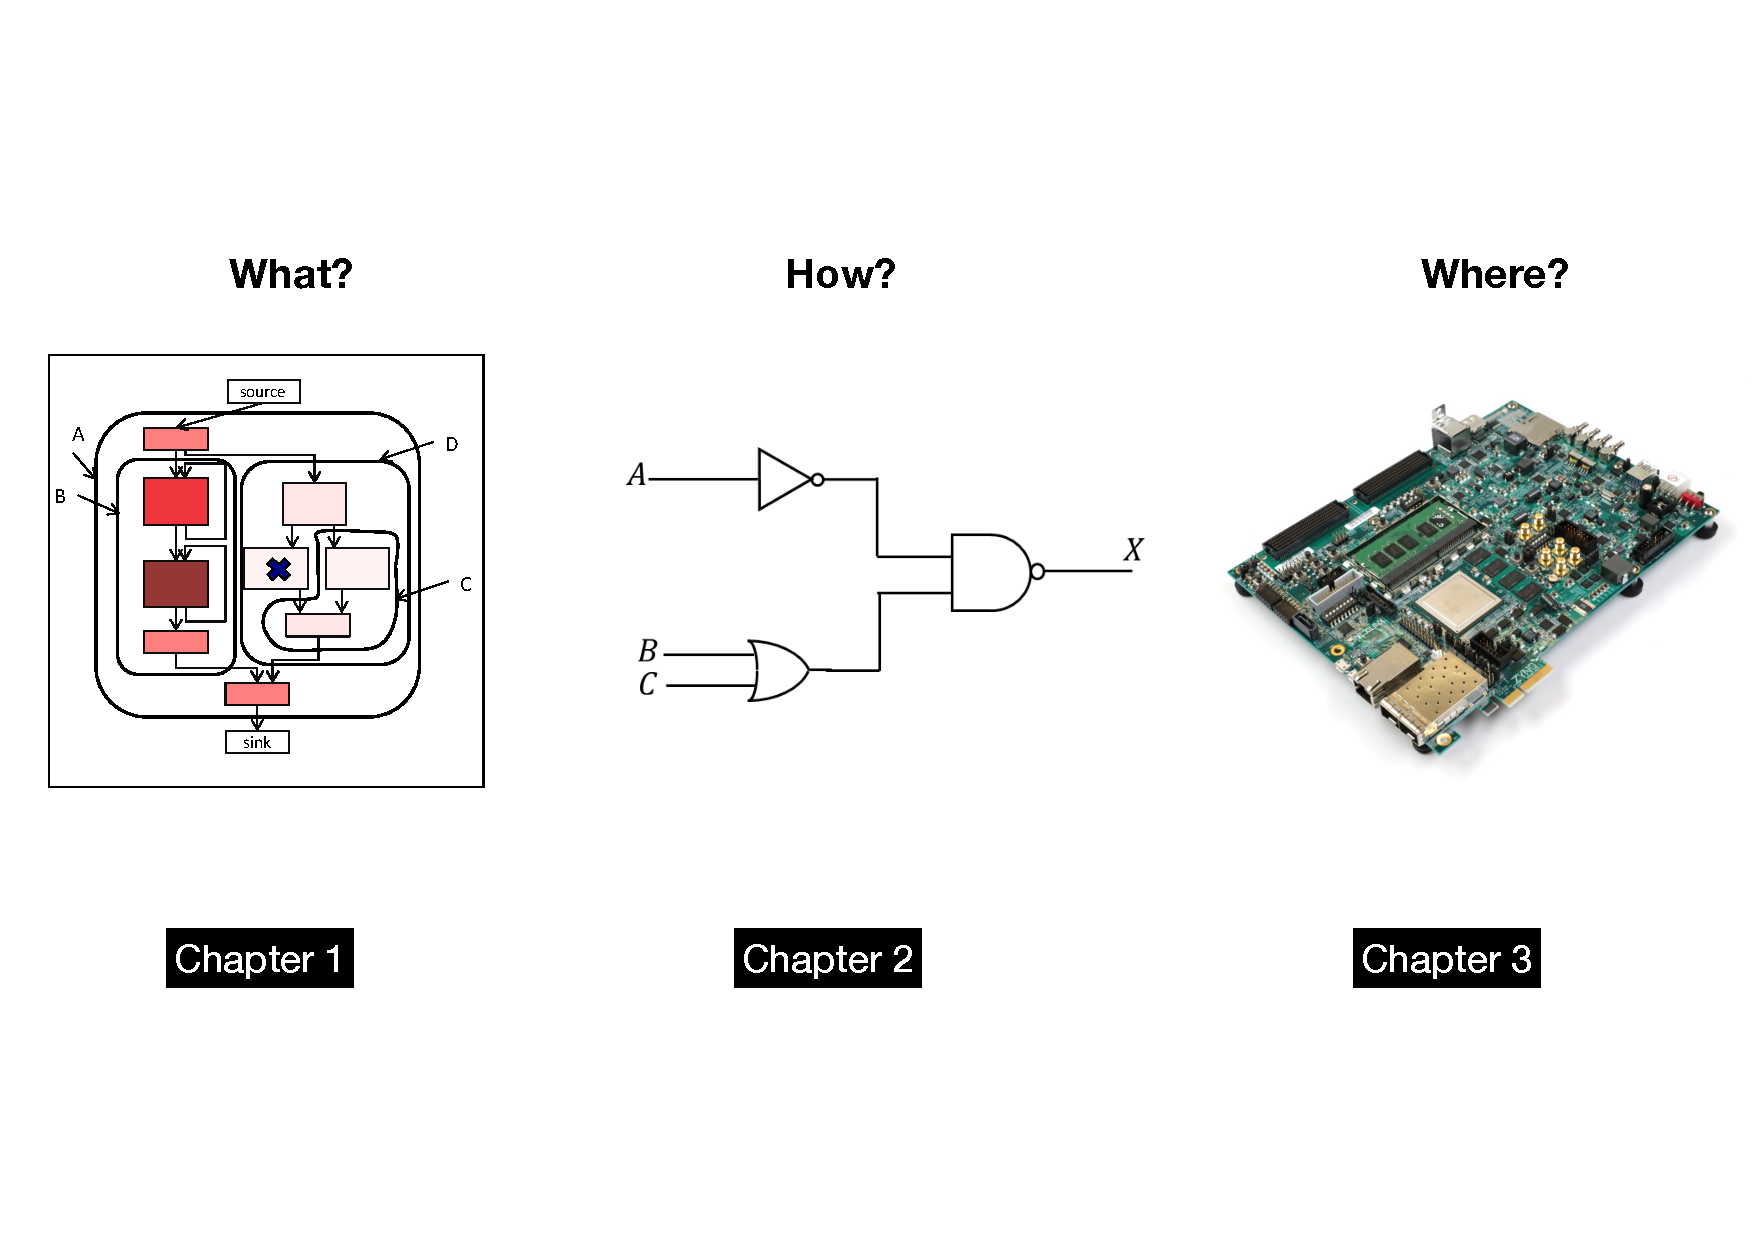
\includegraphics[width= 1 \linewidth]{figs/Research_Carol}
% a figure\dots
\caption{Overview of the research that has been conducted during my PhD and the respective chapters
of the PhD thesis.}
%\vspace{-0.5cm}
\label{fig:overview}
\end{figure}

An overview of the research conducted during my PhD is depicted in Figure \ref{fig:overview}.
This can be viewed as a map of this PhD thesis in order to navigate throughout my 
research time-line and present a high level view of how each piece is connected to each other.\par

Chapter 1 answers the question of {\em what} should be accelerated, namely which parts of 
computation, given a constraint on HW area resources. 
Under the scope of this chapter the \rseeker\ tool-chain is presented \cite{ZacharopoulosApr19}. 
\rseeker\ is an LLVM based framework 
that, given a SW application provided as input, identifies and selects, in a fully automatic fashion, HW 
accelerators under the constraint of an area (HW resources) budget. The granularity of the candidates for 
acceleration considered is that of a subgraph of the control flow graph of a function, with a single control 
input and a single control output. These candidates are called regions. After identification takes place, a selection algorithm solves the problem optimally of 
finding the subset of the initial regions list that, under a given area constraint, maximizes the collective 
speedup obtained. The evaluation of \rseeker\ took place by using both an industrial tool, such as Xilinx
Vivado HLS \cite{VivadoHLSMar17}, and a research HW accelerator simulator, such as Aladdin \cite{ShaoJul14}. 
Experiments carried out with these tools revealed an improvement of performance compared to the \SoTA\
and a speedup gain of up to 4.6x. 
\par

In Chapter 2, the 
analysis that is presented attempts to answer the research question of {\em how} the identified and 
selected HW accelerators should be implemented in order to achieve improved performance. 
Under that scope, Data Reuse analysis, during the execution of a specific domain of applications, 
reveals the effectiveness of private local memory structures \cite{ZacharopoulosJan17}. 
Furthermore, for HW accelerators that contain loops, an optimal
Loop Unrolling factor can be predicted for each of the included loops \cite{ZacharopoulosJul18}. 
The most suitable Loop Unrolling factor
for each loop is defined according to the target of optimization, which can be either less use of HW
 resources or better speedup. With the aid of a prior LLVM based analysis 
 of the loops and Machine Learning classification, predictions can be performed on a set of loops and the respective 
Loop Unrolling factors may be subsequently applied during the synthesis phase of the accelerators. \par

Finally, Chapter 3 tackles the research question of what should be accelerated but at the same time
taking into account {\em where} the specialized HW is hosted.
An analysis of the system at hand and its memory hierarchy can affect vastly the selection
of HW accelerators and subsequently the performance achieved. Latency due to data exchange
between the HW accelerators and main memory could add a significant overhead to the overall 
computation time. In this chapter \aseeker, an LLVM based tool-chain, is presented. \aseeker\ 
performs thorough analysis of applications
and estimates memory latency along with computational latency of candidates for acceleration. The 
granularity of the candidates for acceleration is that of a subgraph of the entire call graph of 
the application. 
%with a root function (node) and zero outgoing edges of the identified subgraph. 
HW accelerators are selected by an algorithm so that speedup, or energy efficiency, is maximized, 
under a given area budget. The evaluation 
of \aseeker\ took place on Zynq UltraScale platform by Xilinx, considering a demanding and complex 
application such as \htsf. With respect to methodologies based on profiling information \aseeker\ 
attained an improved performance with an up to 2x speedup.\\
Automating a complex process, such as the design and implementation of heterogeneous systems, while
improving performance in these systems is the broad goal of this PhD thesis. All chapters of this document 
attempt to provide a step closer on attaining this goal and expanding the \SoTA, as well as opening 
new paths to future work.

% \lipsum[1-4]

%
%
%
%
%  
%     CHAPTER 1
%
%
%
%
%

% \chapter[Short title]{A chapter title which will run over two lines --- it's for
%   testing purpose}
\chapter%[Automatic Identification and Selection of HW Accelerators]
{Automatic Identification and Selection of Accelerators}

Moving towards a heterogeneous era, HW accelerators, dedicated to a specific task, can
improve both speedup of execution and energy efficiency in comparison to a general 
purpose CPU or a set of homogeneous CPUs. Nonetheless, the identification and selection 
of which parts of the computation are to be implemented in HW is a complex and demanding task. 
A thorough understanding of the application to be accelerated is necessary, the HW resources
(area) budget is often tight and the granularity of the candidates for acceleration 
can dramatically affect the overall execution time. Furthermore, optimizations may be applied
to a given, identified HW accelerator and this would produce multiple versions of equivalent
computation instances that can result in various heterogeneous architectures with different
characteristics and, as a result, different performance gains.
In order to address all these issues I present an automated methodology
that receives as input the source code of a given application and outputs a number of 
HW accelerators to be considered for acceleration. Among these candidates a selection takes 
place that maximizes collective speedup, given a HW resources (area) constraint. Finally, 
multiple versions of the same candidate can be considered during the selection phase as well.

\section{Motivation}
\label{sec:mot}


\begin{figure}[t]
\centering
%\hspace*{-2cm}
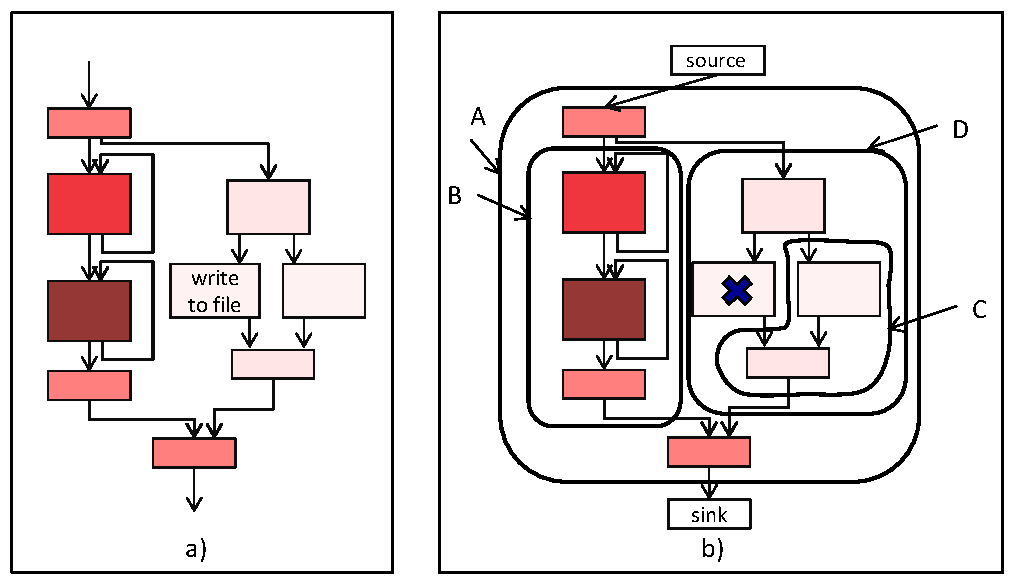
\includegraphics[width= .7 \linewidth]{Figs/cfg_example}
\caption{a) Example \CFG\ of a function, color-coded with frequency
  of execution (the darker the basic block, the more frequent). b) B
  and C are Valid Subgraphs; A and D are not Valid Subgraphs because
  they contain a forbidden node. B is also a CFG region, because it has a
  single \controlflow\ input and output.}
\label{fig:cfg-example}
\end{figure}


What is the rationale behind designer choices, when manually choosing
application parts to be accelerated in HW, and how can those choices
be replicated by an automated tool instead? Although it is possible,
perhaps, that \emph{all} of a designer's rationale cannot be
replicated automatically --- potentially because it requires a deep
knowledge of the application at hand --- it is certainly still
desirable to identify at least a subset of the actions that can be
automated.\par

Typically the designer aim will be: given an available accelerator
area, extract as much as possible of the computation, under the
constraint to require no more than that area, in order to maximize the
resulting speedup.\par 

Under the scope of this research I identify subgraphs of the \controlflow\ 
graph that have a single input control point and a single output control point, 
which herein will be called \emph{regions}, as good candidates for 
acceleration. The rationale
is that these subgraphs have a single entry point, and this
corresponds to the moment of execution when the accelerator is called,
and a single exit point, hence duly returning to a single location in
software when the accelerator is done. Note that this type of
\controlflow\ subgraph has been previously proposed and explored in
compiler research --- under the name of \emph{SESE} (Single Entry
Single Exit) in~\cite{AguilarJune16}, \cite{JohnsonJun94}, and under
the name of \emph{Simple Region} in an LLVM
implementation~\cite{LattnerMar04} --- with the aim of improving the
quality of \emph{SW code generation}, and as a scope for applying
compiler optimizations and parallelization. The idea of
identifying the same type of subgraph is borrowed and applied here in a 
novel way and to a different scenario and aim: that of automatically 
selecting HW accelerators.\par

A motivational example is provided in Figure~\ref{fig:cfg-example}a,
which depicts the CFG of an example function, color-coded with
frequency of execution (the darker the basic block, the more
frequent). A possible choice, when \emph{manually} identifying
accelerators, is to work at the granularity of functions: implement,
in HW, the function most frequently executed. However, this choice
might not be ideal, as the downside can be twofold: 1) a part of a
function might be less frequently executed than other parts (the right
side of the CFG, in the example in Figure~\ref{fig:cfg-example}a),
therefore effectively wasting accelerator real estate. 2) a part of a
function might contain non-synthesizable constructs --- such as the
``write to file" system call in Figure~\ref{fig:cfg-example}a or a function 
call that cannot be inlined.  On the
other side of the spectrum, choosing simply within the scope of single
basic blocks --- therefore, the body of the frequently executed loop
in the picture --- may not be ideal either, as the accelerator will be
called once in every iteration of the loop, which may results in a
large overhead. Furthermore, some speedup potential might be missed,
as larger CFG regions might expose better synthesis optimizations.\par

CFG regions are proposed therefore as candidates for
accelerators considering a granularity that can go from a
single loop to an entire function, and anything in between. 
The main body of my research for this work is the consideration 
of CFG regions as candidates and a method to 
automatically identify and select these regions.

\section{Related Work}
\label{sec:rw}

Automatically identifying parts of computation to be
accelerated is often called, in literature, Instruction Set Extension
identification, or also HW/SW Partitioning. The distinction that is most 
relevant, for this research work, is the
\emph{scope} at which the suggested techniques perform identification: 
identifying accelerators or custom instructions at the \dataflow\ or
the \controlflow\ level.\par

%\subsection{Data Flow Level}
\emph{Data Flow Level}.
\SoTA methods have been
published in literature in order to automatically identify,
\emph{within a single basic block}, the subgraph of \dataflow\ 
according to varying architectural constraints and maximizing speedup
when implemented in HW as a custom instruction. A non-extensive list
include works \cite{YuSep04}, \cite{PozziJul06}, \cite{ChenFeb07},
\cite{ReddingtonAug09}, \cite{GiaquintaMar15} and \cite{MartiFeb12},
where the problem of identifying subgraphs under convexity, I/O
constraint, and/or area is tackled; in \cite{VermaOct07} and
\cite{PothineniJan07} the I/O constraint is relaxed, to be regained
via I/O serialization~\cite{PozziSep05}, \cite{VermaOct07},
\cite{AtasuApr07}, \cite{AhnJan13}. In \cite{CongFeb04} the focus of
the identification process is also on DFG nodes within single basic
blocks, and the constraints that are taken into account are a limited
number of read and write ports, and area.  The methodology proposed in
\cite{GaluzziOct06} is not limited by I/O in the selection process,
but clusters MAXMISOs \cite{AlippiMar99} in order to form MIMOs 
(Multiple Input Multiple Output instructions) that can be executed as 
a single instruction.\par

In none of the above pieces of research, though, the inclusion of the
\controlflow\ of the application is considered during the
identification process. The technique proposed in Section \ref{sec:rs}, 
instead, pushes 
identification \emph{beyond} the basic block level and identifies 
entire regions of the \CFG\ of the
application as candidates for acceleration. Compiler
transformations such as if-conversion and loop-unrolling can be, and
are, used by several of the techniques mentioned above in order to
enlarge the scope of within-basic-block identification, by enlarging 
themselves. Nevertheless, the scope remains limited to those
techniques and cannot include \emph{all} kinds of
\controlflow.\par

\emph{Control Flow Level.}
A smaller amount of research has looked into
identification within CFGs. In \cite{ZuluagaJul09} it is
proposed to implement CFG regions with multiple control exits as
accelerators. However, the presence of multiple control outputs
significantly complicates the processor-coprocessor interface, as
opposed to a single-entry single-exit approach. 
Another paper proposing HW/SW partitioning~\cite{BaleaniMay02}
presents a clustering methodology that operates on a control-data
network compiled from an Extended Finite State Machine (EFSM)
model. While it targets \controlflow\ to a certain extent, their
methodology is limited to applications that can be modeled using
EFSMs, therefore considering a much more limited scope than that of
generic Control Data Flow Graphs compiled from source code, as the methodology
proposed in Section \ref{sec:rs}.

Finally, the authors of a recent work \cite{AguilarJune16} consider
Single Entry Single Exit regions but their target is to identify
strictly parallelizable loop regions and offload them to an MPSoC
target platform. This approach is limited in
terms of excluding non-parallel regions from being potential
candidates to be accelerated, and also in terms of not being cost-efficient, in case a
designer needs to set a specific area constraint for the accelerators.

%\subsection{Compiler Transformations}
\emph{Compiler Transformations}.
Within compiler research, it is fairly 
common to identify CFG subgraphs for code
optimization reasons. For example, trace scheduling, superblock and
hyperblock scheduling~\cite{HankSep93}, identify regions
of the CFG in order to perform global code scheduling and
improve code generation. \emph{SESE} (Single Entry
Single Exit) regions have been proposed in~\cite{JohnsonJun94}, and
their identification was reimplemented in the LLVM framework in an 
analysis pass
called \emph{RegionInfo}, for the purpose of improving the
performance of code generation. For my SW analysis, the idea of
CFG region identification was borrowed from compiler research and was 
applied to automatically identify and select HW accelerators.

\emph{Application Specific Instruction set Processor (ASIP) architectures and design practices}.
HW Accelerators that are embedded
in an Application Specific Processor can be either developed as hardwired
Integrated Circuits (ICs), or mapped onto reprogrammable systems. In the
first scenario, examples of Application-Specific Integrated Circuit (ASIC) 
platforms exist, such as the
Tensilica Xtensa from Cadence \cite{TensilicaMar17} and the ARC
processor from Synopsys \cite{ArcDec16}. These tools can be extended with
accelerators and complex instructions. The CPUs can be configured
during the design process to maximize performance and efficiency,
without enduring the overhead of reconfiguration. An alternative, not 
as performing yet more flexible, is offered by FPGA-based
Systems-on-Chip (SoC) examples, such as Altera (the Arria10 family \cite{ArriaNov16}) and
Xilinx (the Zynq SoCs \cite{ZynqMar17}).\par

The instances mentioned above support the generation of HW
circuits, but do not provide implementation paths for differentiating the
execution between HW and SW. Conversely, High Level
Synthesis (HLS) tools allow designers to move parts of applications, 
written in C or C++, between processors and
accelerators. Research endeavors in this domain include LegUp
\cite{CanisSep13} and ROCCC \cite{GuoMar05}, while commercial
applications comprise the Vivado\_HLS \cite{VivadoHLSMar17} suite
from Xilinx (for FPGAs) and StratusHLS \cite{StratusHLSApr16} from
Cadence (for ASIC development).
However, these HLS frameworks place the responsibility of
partitioning a SW application on the application developer.\par

\section{The RegionSeeker Framework}
\label{sec:rs}

The RegionSeeker framework is an automated methodology that 
identifies candidates for HW acceleration from application C 
code. An extensive SW analysis, based on the LLVM compiler infrastructure,
performs, apart from
the identification, an estimation of the performance gain, along with
the HW resources cost, of each candidate. Subsequently given a HW resources
constraint, a selection of the identified HW accelerators takes place that
maximizes the cumulative performance gain.
In the following subsections the methodology is presented in detail, as well as
experimental results from the CHStone benchmark \cite{HaraMay08} suite.

\subsection{Methodology}
\label{subsec:meth}

There are three parts comprising the methodology, detailed as follows.
The first step is to automatically identify valid regions that are suitable candidates
for HW acceleration. Secondly, an estimation of their potential merit, in terms of cycles saved
(the difference between SW and HW execution cycles),
is computed along with the respective cost, which is the HW resources (area) required
for each region. Finally, a selection algorithm is utilized in order to optimally solve the 
problem of selecting a subset of these
regions that maximize the accumulated merit under a given cost, i.e., an area constraint.

\subsubsection{Region Identification}
\label{subsec:reg_id}

To identify regions in both an automatic and efficient way, a
 \emph{Region Identification} pass was developed under the version 3.8 
of the \emph{LLVM Compiler framework} \cite{LattnerMar04}. 
The pass receives as input applications developed in C or C++ and performs 
their analysis at the Intermediate Representation (IR) level, a type
of code used internally by LLVM to represent source code and allow
data flow analysis and optimizations.\par

The pass iterates over every function of an
 application and, using the existing \emph{RegionInfo} LLVM pass 
\cite{GrosserApr12}, identifies regions within every function.
%, as seen in Figure \ref{fig:region}. 
Subsequently, nodes that cannot be synthesized, such as system
calls or calls to functions that are not inlined, are identified 
and labeled as forbidden.
%forbidden nodes inside regions are identified and labeled, such as system
%calls or calls to functions that are not inlined. 
The regions containing
these nodes are marked as invalid. Conversely, the valid regions are 
evaluated by a profiling-via-instrumentation routine.
Profiling via
instrumentation requires generating an instrumented version of the
code, which gives more detailed results than a sampling
profiler. 
The output of the profiling is a file that contains information regarding 
the execution frequency of each basic block and the total number of calls to each 
function, i.e., the execution frequency of each function.
Using this information, the basic blocks are annotated
 in each function with their respective execution frequency. 
% with the aid of \emph{ClrFreqCFGPrinter} LLVM pass \cite{ZacharopoulosMar17},
 %that I have developed.


% LLVM RegionSeeker Analysis Pass.
% %
\begin{algorithm}[t]
\begin{flushleft}
\textbf{Input:}  Application written in C/C++\\
\textbf{Output:} List of Identified and Profiled Regions\\
\end{flushleft}
\begin{algorithmic}[1]
\Function{$RunOnFunction()$}{}
\State\Call{$Region\_List=NULL$}{}
\State\Call{$RI=getRegionInfoAnalysis()$}{}
  \For {$Region\ in\ Function$}
    \If {\Call{$RegionIsValid()$}{}}
      \State\Call{$EvaluateRegion$}{Region}
      \State{$Region\_List.Add(Region)$}     
    \EndIf
  \EndFor
  \State{$return\ Region\_List$}  
\EndFunction

\State
\State{$/* Estimate\ Merit\ for\ Region*/$}
\Function{$EvaluateRegion$}{Region}
  \For {$Basic\ Block\ in\ Region$}
    \State\Call{$getProfilingInfo$}{Basic\ Block}
  \EndFor
\EndFunction
\end{algorithmic}
\caption{LLVM Analysis Pass - Region Identification} 
\label{algo:reg}
\end{algorithm}

\subsubsection{Merit and Cost Estimation}
\label{subsec:mer_cost}

The Region Identification pass, apart from the Region Identification detailed above, 
performs an early evaluation of the merit and cost of a region, implemented
directly within the LLVM tool-chain. The evaluation relies on the LLVM intermediate
representation and does not need any manual modification to perform function out-lining
on the benchmark source code. 
The estimation of merit and the cost of a region is performed as follows.\par

\emph{Merit Estimation.} 
The merit of a region is defined as the total number of cycles saved in a HW accelerator 
implementation compared to the respective SW implementation of the same piece of runtime 
of a given application. Therefore the merit of a HW accelerator is estimated as the 
difference between the \HW\ and \SW\ run time, across all its invocations in an application,
taking into account the invocation overhead of calling a HW accelerator in a specific 
heterogeneous architecture. The estimation of the HW run time is computed first in the 
basic block (BB) level as the the critical path of the latency (in clock cycles) of the Data 
Flow Graph (DFG) nodes. Runtime profiling information is used in order to determine the execution 
frequency of each BB.
Subsequently the delay of the entire region in HW is estimated by multiplying the critical path
delay of each BB with the respective execution frequency and finally summing up the products, 
according to the specific BBs that comprise the region.
Software run-times are estimated in a similar fashion, but instead of computing critical paths 
at the BB level, the sum of the latency (in clock cycles) of all its constituent operations is 
computed, modeling that these are processed sequentially in software.\par

\emph{Cost Estimation.} On the other side of the evaluation, the cost of a region 
is estimated as the area (or HW resources) required to implement its DFG nodes. The area 
is computed as the sum of look-up tables that is required for
the DFG nodes of the respective HW accelerator. Each DFG node may take up a different amount
of loop-up tables according to its complexity. The characterization for each DFG node was carried
out with the aid of Vivado, a commercial \HLS\ tool, targeting a Virtex7 FPGA.\par
% and its merit as the cycles saved between SW
% and HW execution, where the latter is the delay of the nodes on the
% DFG critical paths. Runtime profiling information is used in both SW and
% HW latency estimations in order to determine the number of invocations for
% each candidate.\par
The final output of the analysis pass is a list of valid regions, 
or else accelerator candidates, each annotated with an estimated merit and cost.
The region list output is in turn processed by the 
\exact\ selection algorithm implemented as standalone program in C++.
% selection algorithms exact and greedy implemented as standalone programs in C++.


\subsubsection{Region Selection Algorithm}
\label{subsec:sel_algo}

Given a merit $M()$ and cost $C()$ function for each region 
we can formulate the problem of selecting accelerators as follows:\\
\textbf{Problem: Region Selection}
Let $\mathcal{R} = \{ R_1, R_2, \ldots, R_n \}$ be a set of regions,
with associated cost and merit functions $C$ and $M$.
For any subset $X\subseteq \{1,2,\ldots,n\}$ of regions,
we denote by $M(X) = \sum_{i\in X} M(R_i)$ the sum of the merits of
its regions, and we denote by $C(X) = \sum_{i\in X} C(R_i)$ the sum of
the costs of its regions.

We want to select a subset $X$ of regions such that
\begin{enumerate}
\item No two regions belonging to the same CFG overlap, i.e.,
  $V(R_i)\cap V(R_j) = \emptyset$, for all $1\le i,j\le n$
\item The cost $C(X)$ is within a user-given cost budget $C_{\max}$
\item The merit $M(X)$ is maximized
\end{enumerate}


This problem definition maps to what we have identified in
Section~\ref{sec:mot} as the designer aim: given an available
accelerator area, extract as much as possible of the computation,
under the constraint to require no more than that area, in order to
maximize the resulting speedup.\par

\begin{figure*}[t]
\centering
%\includegraphics[width= \linewidth]{figs/figs_from_pptx/exact_tree.pdf}
\includegraphics[width= .9 \linewidth]{Figs/exact_tree.pdf}
\caption{Tree exploration performed by \exact, for the running example
  of Figure~\ref{fig:cfg-example}, and for a cost budget of 35.}
\label{fig:exact_tree}
\end{figure*}

An exponential, \exact\ branch-and-bound method
based on a binary-tree search was derived in order to solve optimally 
the Region Selection problem. The algorithm converges to an
% is implemented so that it finds the 
independent set of regions that maximizes merit under 
a given cost.
This process can be exemplified through
 Figure~\ref{fig:exact_tree}: given an initial set $P$, that includes all
 valid regions identified, and a set $X$, that is initially an empty set and 
is going to be the subset of $P$ that maximizes merit under a given cost.
The root of the tree represents the empty set, and set $P$ at this
point contains all regions. Furthermore an overlapping graph among regions 
shows whether there is overlapping among valid regions contained in $P$, 
such that it poses the restriction of not allowing the selection of regions 
that overlap with each other, i.e., containing at least one BB that is common. 
The overlapping graph is seen as well in Figure~\ref{fig:exact_tree}.
As the algorithm starts the exploration, inclusion of region A is first
considered, and the set P is updated by removing all regions overlapping
with A: $P = \{E\}$. According to the merit and costs of all regions
in this example, shown in the table within the picture, the merit (60)
and cost (35) of the solution currently explored is also updated.\par

At every point of the exploration, a new node $u$ is considered for
addition in the current independent set.
If there is no node $u$
satisfying condition $2$ of the Region Selection Problem, the algorithm
records the set $X$ and backtracks, as $X$ is maximal with respect to
condition $2$.  For the running example in
Figure~\ref{fig:exact_tree}, the cost budget $C_{\max}$ is equal to
$35$. Hence, exploration stops at $X=\{A\}$ because the cost budget
has been reached, and backtracks. The next region chosen is $B$, sets
$X$ and $P$ are again updated accordingly, to $X=\{B\}$ and
$P=\{C,D,E\}$, and exploration continues until the selection algorithm
converges.\par

Two optimizations are implemented in the exact selection algorithm in order 
to avoid unnecessary exploration. Optimization 1 performs a look up in order 
to determine whether the maximum recorded merit can be reached by the 
regions contained in $P$ or not. If not the exploration stops and backtracks.
Optimization 2 ranks the valid regions in terms of merit so that the first 
region considered for inclusion in $X$ is the one with the maximum merit.


\subsection{Experimental Results}
\label{subsec:exp}

% The evaluation of the \rseeker\ framework took place by 
% retrieving the HW execution latency, 
% as well as the HW area resources, using the Xilinx Vivado\_HLS tool-suite.
% Vivado\_HLS outputs are intended for FPGA designs. Synthesis within this
% framework provide exact latency (number of cycles)
% and area (Look Up Tables and Flip Flops) values of each accelerator.\par

The evaluation of the \rseeker\ framework took place by 
assuming a system constituting a single SW processor and multiple HW accelerators, 
exchanging shared data with \plms.
The processor activates the accelerators via a memory-mapped
interface, thus requiring a transaction on the system bus. 
When activated, accelerators read and
write data to and from the \plms, computing their outputs, which
can then be accessed by the processor. Accelerators are interfaced to \plms\
with ports having a latency of one clock cycle. The
control interface between the processor and the accelerators was modeled 
with a
latency of 10 clock cycles.\par
% These parameters correspond to the ones
% employed by the \texttt{ap\_memory} and \texttt{s\_axilite}
% interfaces, respectively, provided by Xilinx Vivado.\par

The run-times of the non-accelerated SW part of the considered
benchmarks were measured using the Gem5
simulator~\cite{BinkertFeb11}, modeling an ARMv8-A processor with an
issue width of 1. The processor model is atomic, with in-order
execution. It is interfaced with separate instruction and data
memories with an access latency of one clock cycle.\par

Hardware execution times were retrieved using two different HLS 
frameworks: the Aladdin simulator and the Xilinx Vivado\_HLS
commercial tool-suite.  Aladdin targets ASIC implementations.  It
provides a fast evaluation, but does not produce a synthesizable netlist
as output; nonetheless, the estimations offered by this tool are
within 1\% of the ones derived from an RTL implementation
\cite{ShaoJul14}.  Hardware instances generated with Vivado\_HLS are
instead intended for FPGA designs. Synthesis-runs within this
framework are more time-consuming, but provide exact area (HW resources
in terms of Look Up Tables and Flip Flops)
and latency (number of cycles) values of each accelerator, as well as a direct
path to its realization.  In both cases, default implementations of
the accelerators were considered, i.e., no optimizations were applied to the
implemented HW accelerators.\par

The benchmarks that were used during the experimental phase are embedded applications
of varying size from the CHStone benchmark suite \cite{HaraMay08}.
\adpcm\ performs an encoding routine and \aes\ is a symmetric-key encryption algorithm. 
\dfmul\ and \dfsin\ are small kernels that perform double-precision 
floating-point multiplication and sine functions employing integer arithmetics. 
\gsm\ performs a linear predictive coding analysis, used in mobile communication. 
\jpeg\ and \mpeg\ are larger applications, implementing JPEG and MPEG-2 compression, respectively.
Finally, \sha\ is a secure hash encryption algorithm, used for 
the generation of digital signatures and the exchange of cryptographic keys.\par

\begin{figure}[h!]
\centering
\hspace*{-1cm}
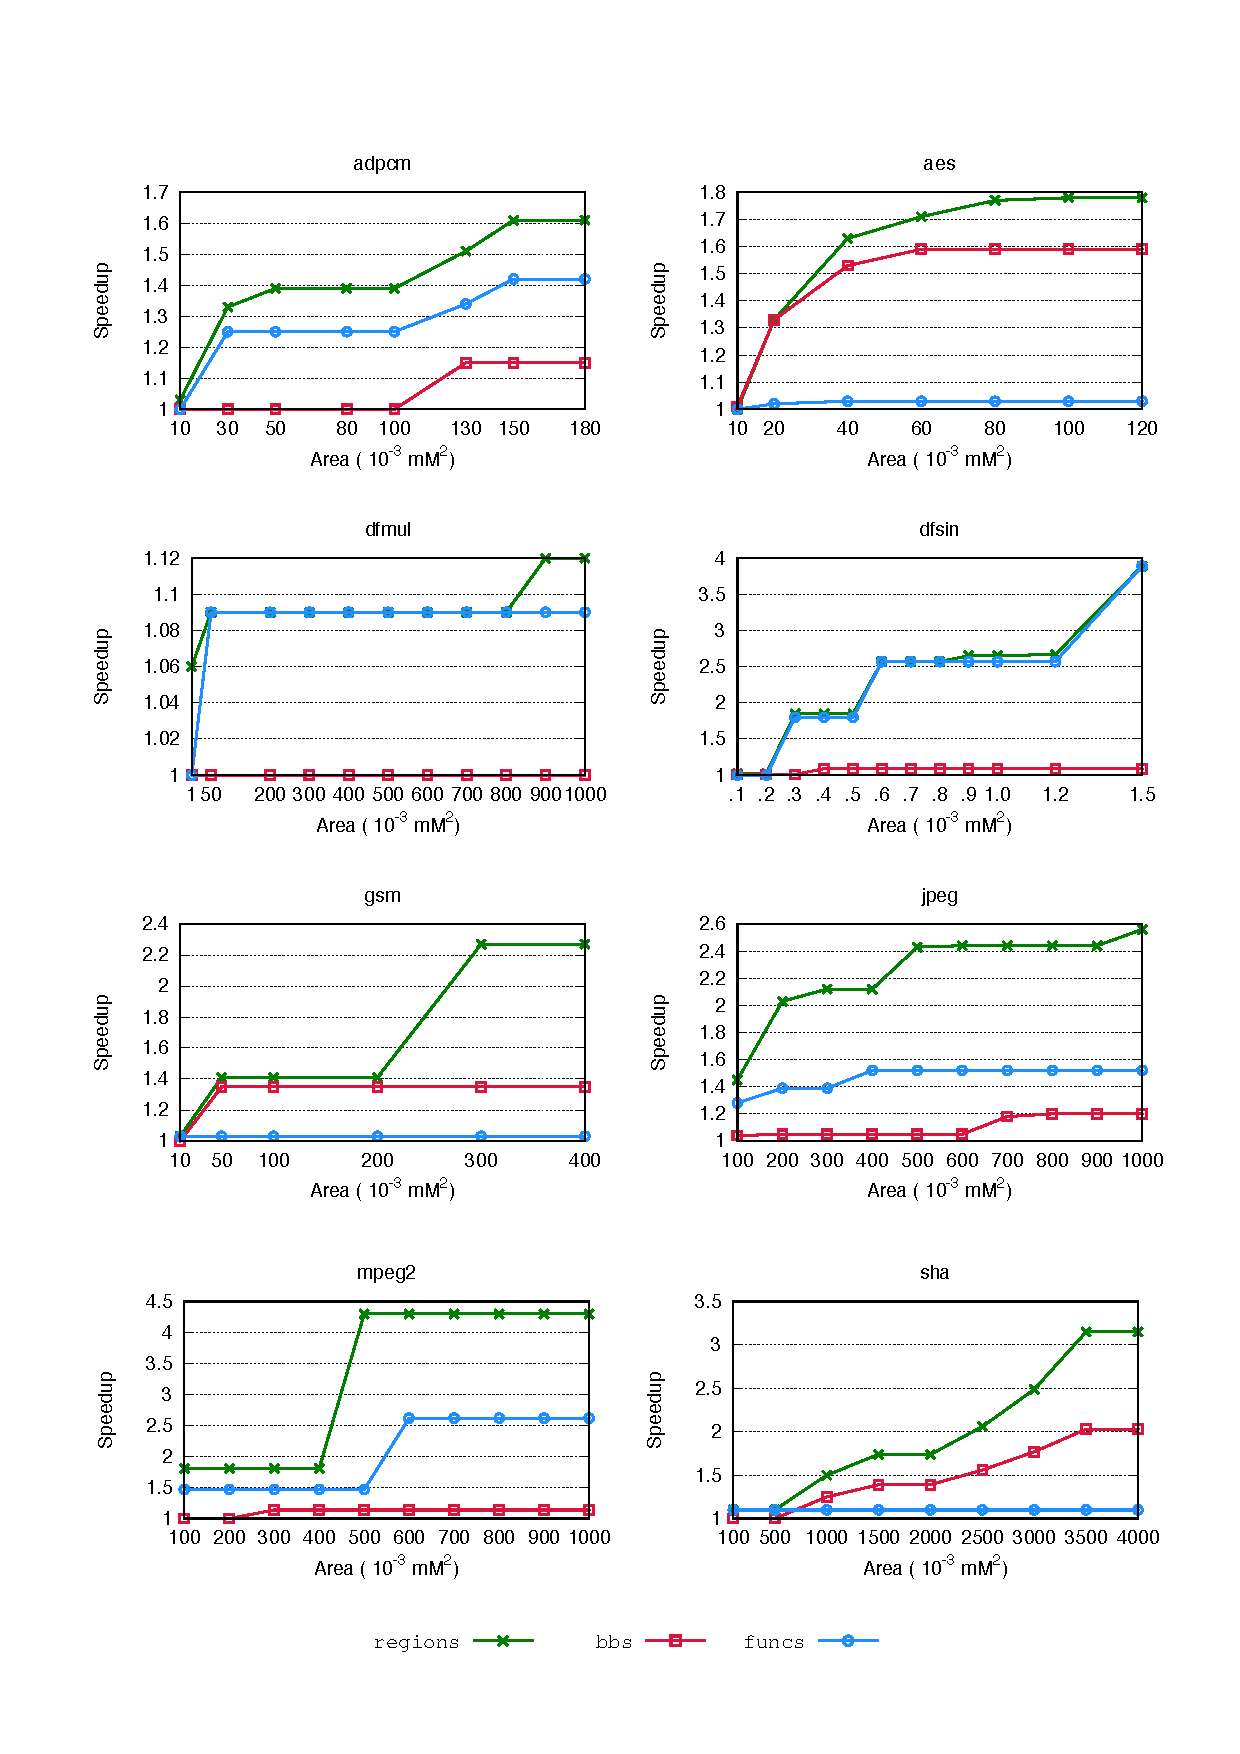
\includegraphics[width= 1.1 \linewidth]{figs/regions_aladdin}
\caption{Comparison of speedups obtained on eight CHStone benchmarks
  by selecting regions, only basic blocks and only functions, varying
  the area constraint, using Aladdin and Gem5 for Speedup and Area evaluation.}
\label{fig:regions_aladdin}
\end{figure}

Figure~\ref{fig:regions_aladdin} showcases the achieved
speedup, when employing Aladdin, by the accelerators selected by
\rseeker\ (labeled \texttt{regions} in the figure), with respect to
the entire run-time of the applications and for different area
constraints.  For small-to-medium size applications such as \adpcm,
\aes, \gsm\ and \sha\ speedup gains for \rseeker\ vary from 1.6x up to
3.2x. For smaller kernels, larger variations can be observed, as for
\dfmul\ and \dfsin\ the speedup reaches 1.12x and 3.9x respectively.
Finally, for larger benchmarks such as \jpeg\ and \mpeg\, speedup is
fairly significant: 2.5x for the former and up to 4.3x for the latter
can be reached using \rseeker.\par

\begin{figure}[h!]
\centering
\hspace*{-1cm}
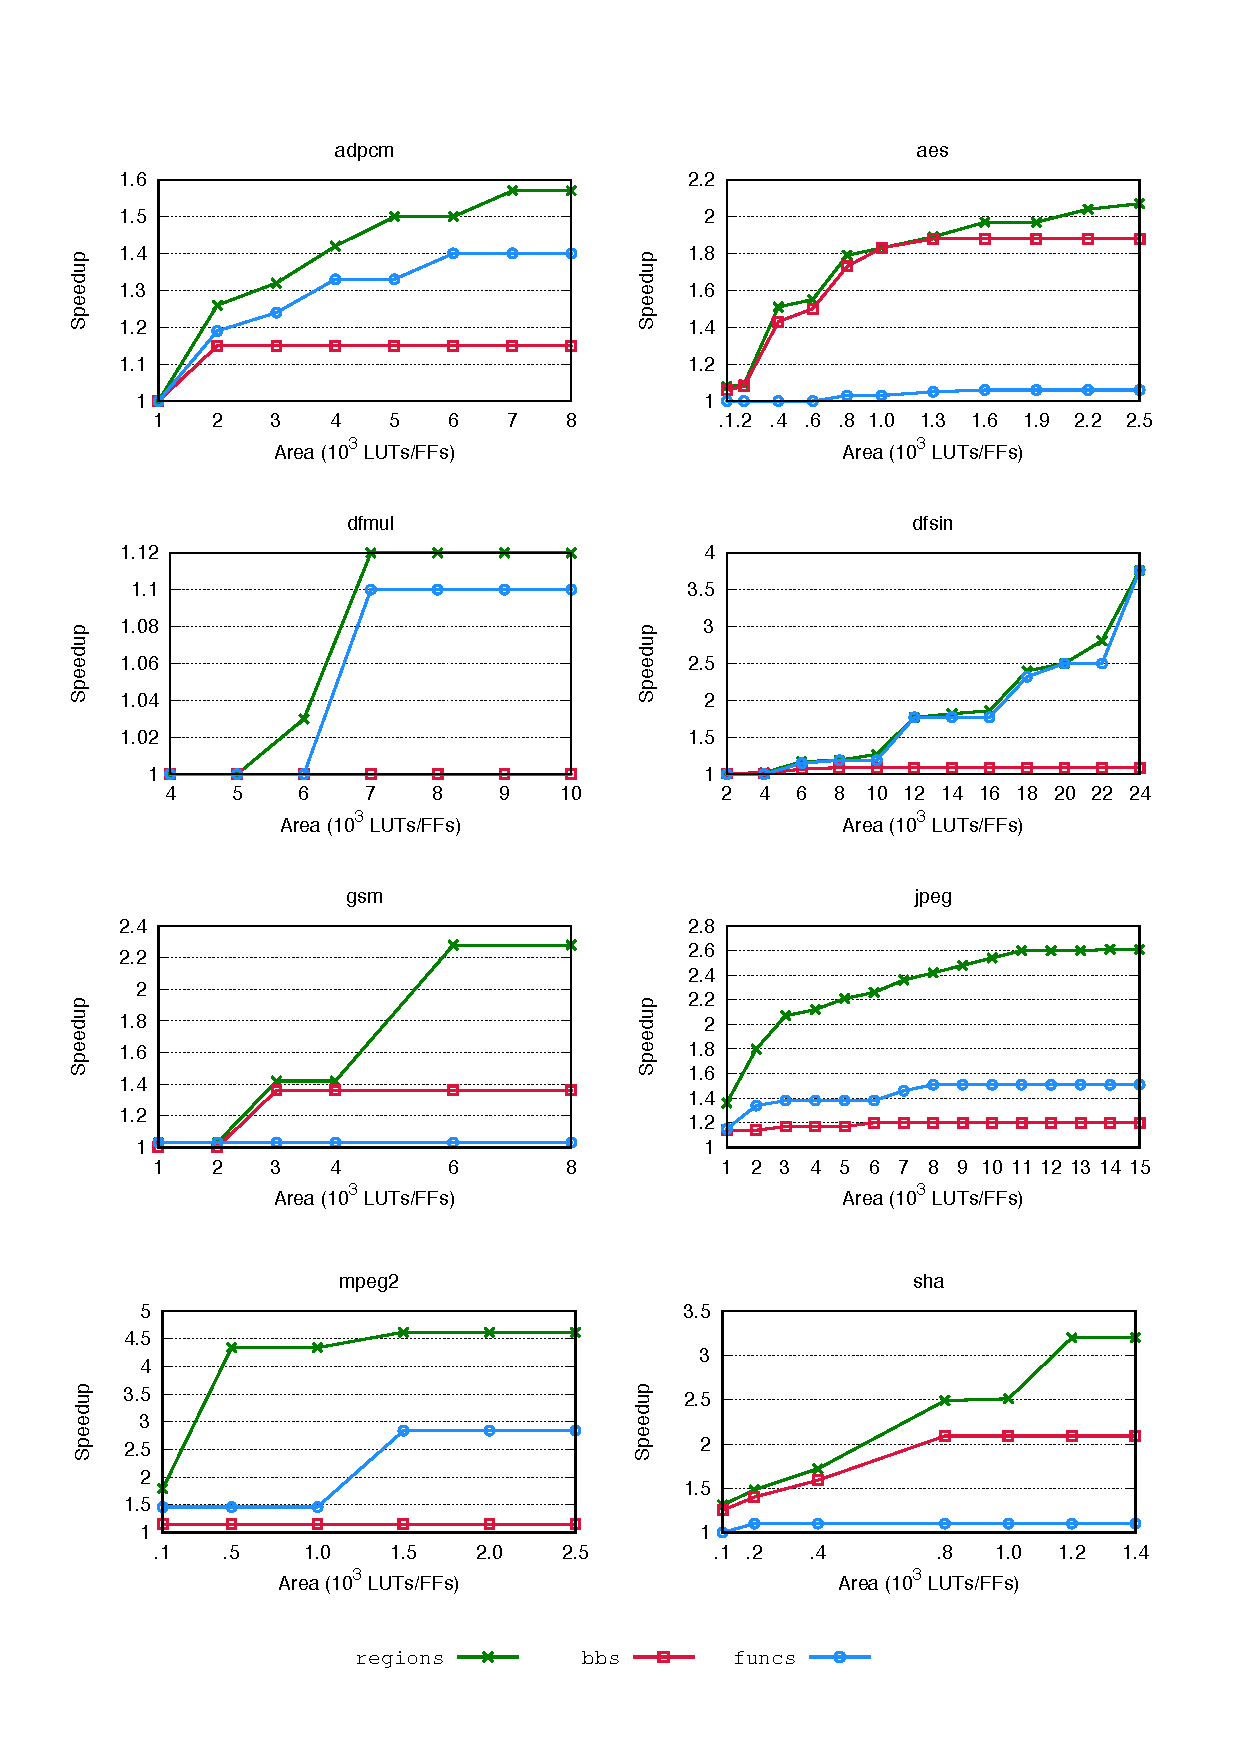
\includegraphics[width= 1.1 \linewidth]{figs/regions_vivado}
\caption{Comparison of speedups obtained on eight CHStone benchmarks
  by selecting regions, only basic blocks and only functions, varying
  the area constraint, using Vivado\_HLS and Gem5 for Speedup and Area evaluation.}
\label{fig:regions_vivado}
\end{figure}

Similar trends are observed when Vivado\_HLS is instead used for the
accelerator synthesis, as reported in
Figure~\ref{fig:regions_vivado}: \rseeker\ consistently outperforms
\SoTA\ approaches which target either single basic blocks or
entire functions, across all benchmarks. These results 
highlight that the achievable speedups
are highly influenced by which segments of applications are selected
for accelerations, and that such choice is only marginally influenced
by the adopted merit and cost estimation tool. In fact, this was verified 
across the two sets of experiments, as the regions chosen were
the same in 80\% of the cases. As an example, out of 10 regions
selected to achieve a 2.2x speedup for the \jpeg\ benchmark, 8 are the
same when using either Aladdin or Vivado\_HLS for merit and cost
estimation, and the ones that differ contribute to less than 14\% of
the provided gain.\par


\begin{figure}[h!]
\centering
%\hspace*{-2cm}
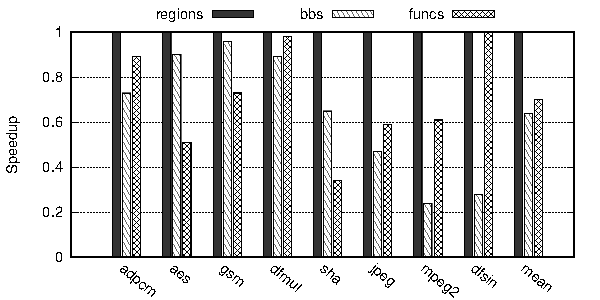
\includegraphics[width= 0.9 \linewidth]{figs/rbf_max_norm_all}
\caption{Normalized Speedup of RegionSeeker with respect to function and basic block selection, 
considering, for each benchmark, a fixed area constraint. Synthesis performed with Vivado\_HLS.}
\label{fig:regions_all}
\end{figure}

Finally, in Figure \ref{fig:regions_all} a summary of the performed experimental 
exploration is presented. It reports the normalized speedups
obtained by \rseeker\ compared to basic block and function
identification, when a fixed area budget is considered and
Vivado\_HLS are employed. The mean column illustrates that,
on average, \rseeker\ achieves approximately 30\% higher speedups
with respect to the two baseline methods. Moreover, while in some
cases the baselines match the performance of \rseeker\ (e.g.: \gsm\
for basic blocks, \dfsin\ for functions), neither of them can achieve that
consistently across applications, stressing the suitability of control-flow regions as
HW accelerator candidates.\par

The speedup that can be obtained by accelerating basic blocks is
hindered by their small granularity and, consequently, the high number
of HW accelerators invocations by the SW processor, i.e., the switches 
between software and hardware execution. Moreover, in this
setting many optimization opportunities
during the hardware implementation of the accelerators are missed,
because they only arise when control flow is considered, as is instead the case
for regions.\par

On the other hand, the speedup derived by selecting whole functions
trails the one corresponding to regions, because of two
reasons. First, function selection is limited to the ones which do not
present forbidden nodes, and this may rule out promising regions
within them. Second and more importantly, it is inflexible from
an area viewpoint, which is especially visible when few hardware
resources are available for acceleration. In those cases, the
selection of functions often detects only few feasible candidates,
with a small merit (e.g. in Figure \ref{fig:regions_aladdin}: \jpeg\ and 
\mpeg, for an area of less than 0.5 $mm^2$).\par

This limitation, though, is not present in regions, as simply the part
referring to individual hotspots inside a function can be available
for selection. Indeed, the performance of \rseeker\ stems from the high
flexibility of the selection approach, as it allows the consideration of
the entire spectrum of granularity ranging from whole functions to
single loops, ultimately enabling a better exploitation of speedup for
a given area budget.


\newpage
\section{RegionSeeker MuLTiVersioning}

\HLS\ (HLS) tools, such as Vivado\_HLS by Xilinx, may employ %additional 
optimizations to HW accelerators
design in order to increase performance, i.e. obtain faster execution. These 
%pragma-directed 
HLS optimizations were not taken into account by \rseeker\ framework in the
previous section. Default, non optimized versions of HW accelerators were identified
and selected instead. In this
section an extended \rseeker\ framework is presented, which performs the selection not 
only among possible CFG subgraphs, but also among different versions of each identified 
subgraph, namely different versions of the regions identified. 
This extension is referred to in the rest of the document as RegionSeeker: the 
MuLTiVersioning approach.

% The \rseeker\ framework, as detailed in the previous section, was designed in order to identify
% the most efficient HW accelerators under a given constraint, but was targeting default HW
% implementations. Pragma-directed HLS optimizations were not taken into account. In this 
% section we present an extended \rseeker\ framework, which performs the selection not 
% only among possible CFG subgraphs, but also among different versions of each identified 
% subgraph of the CFG, namely different versions of the regions identified. 
% We call this extension the RegionSeeker: MuLTiVersioning approach.

\subsection{Methodology}
\label{subsec:mv_meth}

The rationale, supporting the extension of \rseeker\ framework, is to achieve improved
speedup that can be provided by exploiting a more varied set of HW accelerators, with different 
optimizations implemented onto them, to select from. This is being achieved by instantiating 
different versions of each HW accelerator with the same functionality, yet different speedup gains 
and different area (HW resources) requirements. The set of optimizations that were considered in 
order to design different HW implementations of the same accelerators are: 
\begin{enumerate}
\item The Loop Unrolling 
(LU) factor, in accelerators that contain loops.
\item The loop pipelining option, being either on or off.
\item The array partition factor, 
which is the number of input and output ports of the memory buffer (scratchpad) attached 
to the accelerator.
\end{enumerate}\par

Loop unrolling optimization is an HLS directive that, in the context of \HLS\, instantiates multiple 
copies of the logic implementing the functionality defined in a loop body, drastically impacting the 
performance of HW accelerators \cite{KurraApr07} \cite{KulkarniOct12}. This directive can be applied in HW
accelerators containing loops whose trip count can be statically defined. It should nonetheless
be applied in a careful manner, as it entails a high area cost for the duplicated logic. Furthermore,
the resulting benefits can be hampered by loop-carried dependencies and frequent memory
accesses.\par
Loop pipelining is an additional HLS directive applied in loops that allows the pipelining of 
the operations contained in a single body of a loop and across consecutive iterations. Restrictions 
regarding loop-carried dependencies across consecutive iterations can limit the application of the loop
pipelining optimization, as the result of the output of a loop iteration would be required in the following
one, thus not allowing the pipelining of the loop body operations.\par

Given an initial set of HW accelerators, i.e., a set of regions that is derived by the \rseeker\ framework, 
multiple versions for each region can be generated that maintain the same functionality.
Each version may employ one of the optimizations listed above, or a combination of them.
\par


All versions of the HW accelerators were evaluated by exploiting the Aladdin HW accelerator simulator.  
Aladdin targets ASIC implementations. It
provides a fast evaluation, but does not generate a synthesizable netlist,
as opposed to Vivado\_HLS. Nonetheless, the estimations provided are
within 1\% of the ones derived from a Register-transfer level (RTL) implementation, according to 
the developers of Aladdin \cite{ShaoJul14}.
For all simulated versions of the selected regions (or HW accelerators), the number of Cycles and number 
of Functional Units (FU) Area were retrieved. For the SW execution time the gem5 simulator 
\cite{BinkertFeb11}
was used with two CPU settings: a) TimingCPU  (a simple and slow CPU with only two pipeline stages)
and b) O3CPU (a complex and fast CPU with five pipeline stages and other resources such as a 
branch predictor, reorder buffer etc). \par


The \exact\ selection algorithm, as detailed in Subsection \ref{subsec:meth}  was used subsequently to 
perform the optimal subset selection, 
given an initial set of HW accelerators along with their respective versions, as well as a specific 
area (HW resources) budget. An important note is that no more than one version of each candidate 
can be selected, as only one realization of the respective SW execution is required.
To ensure that, the selection took place utilizing the overlapping graph presented in Figure \ref{fig:exact_tree} 
containing the basic block indexes included in each region. As a result the set of basic block indexes for 
multiple versions of the same region would be identical.
Experiments were run in \jpeg\ benchmark and four different selection
approaches are presented, compared to the \multi\ approach.\par

\subsection{Experimental Results}
\label{subsec:mv_res}

The experimental setup was the same as in the \rseeker\ framework, with a system comprising a single 
SW processor and multiple loosely coupled HW accelerators, exchanging shared data with \plms.
The processor invokes the accelerators via a memory-mapped
interface, thus requiring a transaction on the system bus and as soon as the HW accelerators execution is complete,
control returns to the SW processor.\par

The speedup achieved on \jpeg\ benchmark, over the respective SW 
time of the same set of selected regions (kernels) %, and the whole application 
are showcased. 
The four different approaches compared are:
a) the \emph{min} where the regions with the least amount of area are included in the set
and hence can be selected, b) the \emph{base} 
where the regions with median values of area are selected, c) the \emph{max} where only the maximum 
area regions can be selected and finally d) the \multi\ approach where any possible version 
of the regions can be selected. \par

\begin{figure*}[h!]
\centering
\hspace*{-1cm}
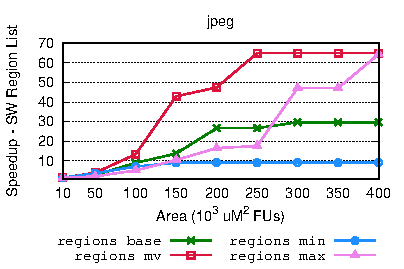
\includegraphics[width= 0.7 \linewidth]{figs/plot_O3CPU_SW_large}
\caption{Comparison of speedup obtained on jpeg benchmark, over the
SW time of the equivalent kernels (regions), varying the area constraint, using 
Aladdin and gem5 for Speedup and Area evaluation.
Four approaches are compared: The 
min where the regions with least amount of area are selected, the base
where the regions with median values of area are selected, the max where 
only the maximum area regions can be selected and finally the \multi\
approach where any version of the regions can be selected.
}
\label{fig:mlv_aladdin}
\end{figure*}

The strength of the \multi\ approach and the benefit of having 
a variety of potential candidates to select from 
%for any equivalent computation, throughout the \jpeg\  application 
is demonstrated by the experimental outcome of the \jpeg\ application (kernels run-time). 
In Figure \ref{fig:mlv_aladdin} for any given area point, the speedup obtained is higher than any other 
methodology. For a medium area point ($200 * 10^3 uM^2$), the 
speedup achieved with \multi\ is 1.7x more than the second best, \emph{base} approach. For 
a large area constraint ($400 * 10^3 uM^2$) the \multi\ speedup is more than 2x compared to
\emph{base} and more than 6x compared to \emph{min}.\par

% In Figure \ref{fig:mlv_speed_aladdin} the same trend is depicted in the speedup of the whole application
% for the MuLTiVersioning methodology, where it constantly outperforms every other competitive method while
% reaching a maximum speedup of 1.8x over the entire jpeg application.\par



% \begin{figure}[h]
% \centering
% \hspace*{-1cm}
% 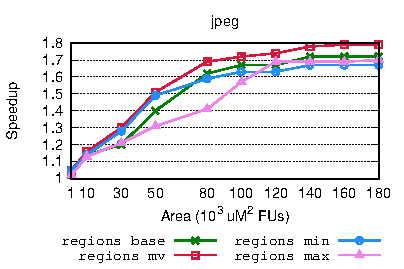
\includegraphics[width= 0.7 \linewidth]{Figs/plot_O3CPU}
% \caption{Comparison of speedup obtained on jpeg benchmark, 
% varying the area constraint, using 
% Aladdin and Gem5 for Speedup and Area evaluation.
% Four approaches are compared: The 
% min where the regions with least amount of area are selected, the base
% where the regions with median values of area are selected, the max where 
% only the maximum area regions can be selected and finally the MuLTiVersioning
% approach where any version of the regions can be selected.}
% \label{fig:mlv_speed_aladdin}
% \end{figure}


\section{Conclusions}
\label{sec:rs_conclusions}

The \rseeker\ framework, along with the \rseeker\ \multi\ extension of the former, are
methodologies that extend the \SoTA\ in the HW/SW co-design domain. They provide
efficient solutions to the problem of automatically deciding which parts of an application should
be synthesized to HW, under a given area budget. The accelerators identified by \rseeker\ 
consistently outperform the ones derived by data flow level algorithms and strictly function 
level candidates, across applications of widely different sizes and for varied area constraints.
As an example, \rseeker\ offers up to 4.5x speedup for the \mpeg\ benchmark compared to as SW
execution. This work was published in IEEE Transactions on Computer-Aided Design of Integrated 
Circuits and Systems (TCAD) journal \cite{ZacharopoulosApr19}.
The \multi\ approach extends the initial selection pool of candidates and, compared
to default HW accelerators configurations, offers enhanced speedup on the \jpeg\ application of up
to 1.7x speedup on the entire application and up to 65x speedup on the relative kernels that 
are synthesized into HW.

% \begin{figure}
% \centering
% 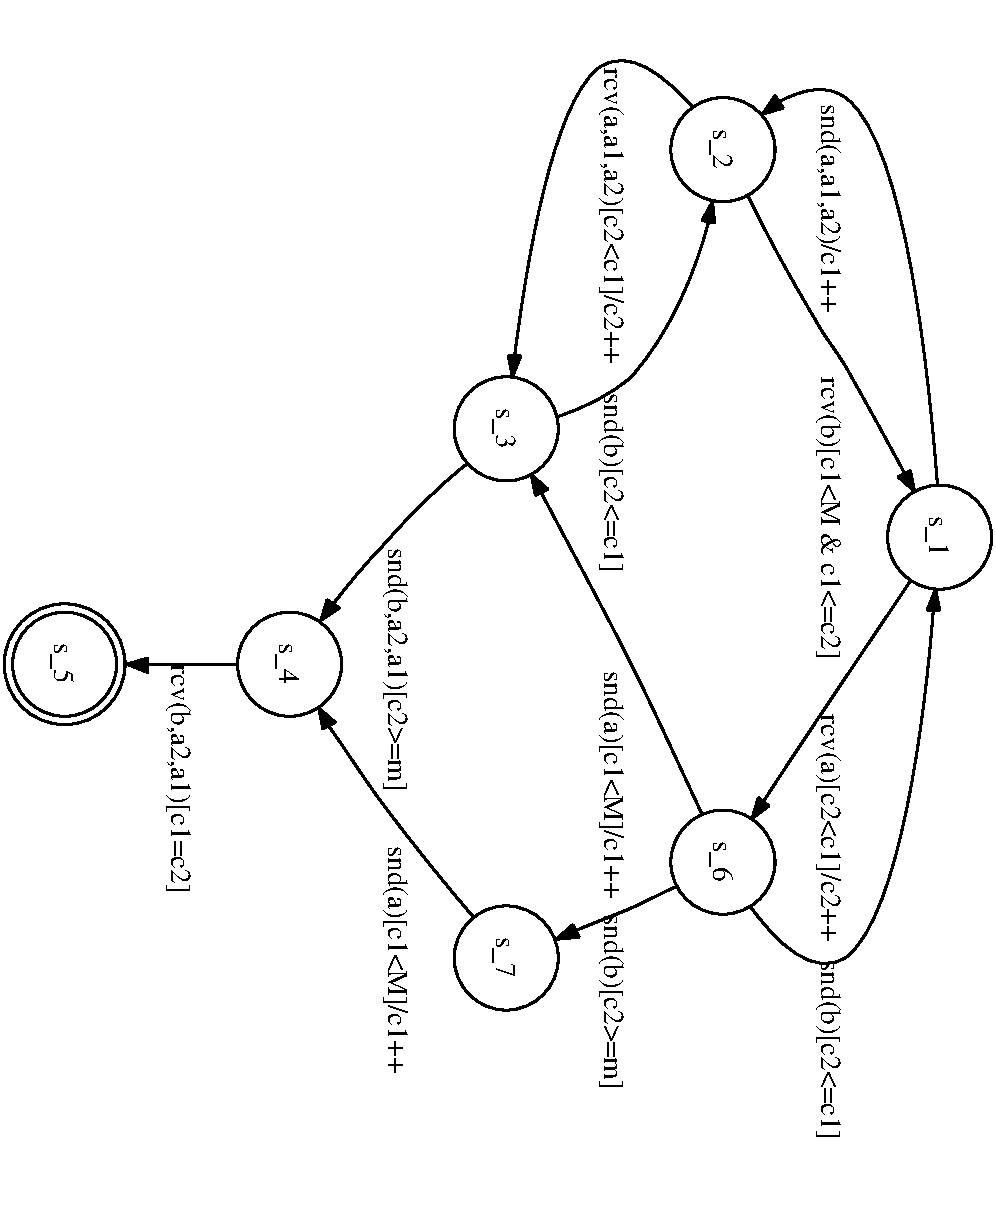
\includegraphics[scale=0.5,angle=90]{bounded_loop_automaton}
% \caption{\textsc{Automaton} for something or other. A caption can be rather
% long and \emph{should} then consist of complete sentences ended with a `.'}
% \end{figure}

% \section{The first \textsc{Section}}

% Here is some text with \textsc{SmallCaps} in normal font.

% \appendix %optional, use only if you have an appendix
% I removed mine a year ago.

%
%
%
%
%  
%     CHAPTER 2
%
%
%
%
%

\chapter{Automatic Optimizations for Accelerators}
% \vspace{-1cm}

Identifying good candidates for HW acceleration is the first step to realize heterogeneous
computing system designs that offer increased performance compared to a homogeneous system restricted
to general purpose SW CPU(s). However, a set of optimizations applied on HW accelerators can decrease 
even more the computational times, thus leading to an improved performance compared to default
non-optimized HW accelerator implementations. 
Modern \HLS\ (HLS) tools can apply such optimizations to 
HW accelerators and increase the performance of their implementations, as well as the overall performance 
of the entire heterogeneous system.
HLS tools such as Vivado\_HLS  \cite{VivadoHLSMar17}, however efficient, though, are far from 
optimal since they require a lot of manual decisions from the programmer's part when it comes to the
choice of {\em how} these accelerators can be synthesized.
Furthermore, the resolution of which optimizations may be applied to which HW accelerators can be a 
complex problem, as it depends heavily on each HW accelerator characteristics.\par

In order to bring automation one step forward in HW/SW co-design, and under the scope of this part of my 
research, I tackled the problem of automating the decision making process of which optimizations should be 
applied to candidates for HW acceleration within a certain context. 
These optimizations include memory management of the data consumed and produced by the HW accelerators, 
a set of optimizations targeted to loops (e.g. loop pipelining, loop unrolling, loop flattening etc), 
pipelining consecutive pieces of computation such as subsequent function calls or loop bodies of consecutive 
iterations and array optimizations, such as array partitioning in blocks of the same size. Among the various 
optimizations available, I have focused on two major categories: a) Data Reuse analysis and b) Loop Unrolling 
factor prediction. Both of these instances are explained in more detail in the following two sections.

\section{Data reuse Analysis}


\subsection{Motivation}

\begin{figure}[h]
\centering
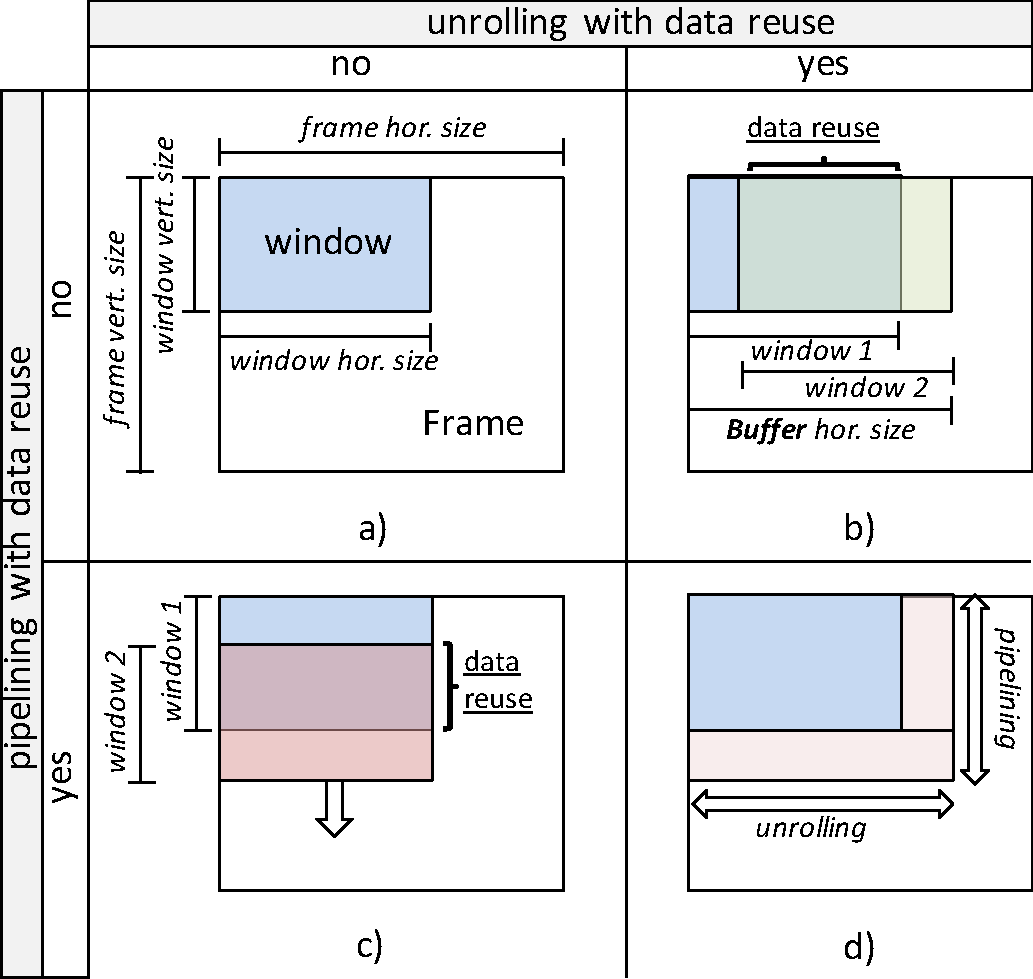
\includegraphics[width= .6 \linewidth]{figs/intro}
\vskip -.5em
\caption{At each iteration, sliding window applications process a
  subset of the input data (a).  The managed set of subsequent
  iterations present a high degree of overlap, both in the horizontal
  (b) and vertical (c) dimensions. The framework in \ref{sec:dr_meth} automatically
  leverages both, maximizing data reuse (d). }
  \vskip -1em
\label{fig:dr_intro}
\end{figure}

Loops are ideal candidates for acceleration. In almost every application, there is a
number of them that contain a large number of iterations and there is a sufficient 
amount of computation taking place in their bodies. In addition to that, there are 
nested loops which commonly show a high level of data reuse. An effective exploitation
of data reuse across consecutive iterations of loops can significantly lower the required
amount of data exchange between HW accelerators and the main memory, thus reducing the 
respective bandwidth to and from accelerators, and increasing their performance.\par

An example of such high
data reuse can be observed in sliding window applications, where there is typically
a window of accesses scanning a wider domain, such as a two-dimensional array. 
Given that the level and pattern of data reuse is known a priori, it is feasible 
to design specific memory structures, also known as memory buffers, attached to the 
HW accelerators. These memory buffers can exploit data reuse by keeping data locally 
and, hence, minimize the memory latency due to communication with the main memory.\par
 %while exploiting the computational potential of the accelerators.\par

Data reuse exploitation in \HLS\ (HLS) is still in premature stage.
\SoTA\ methods \cite{Vivado12} either rely on manually rewriting the source code, preceding HLS, 
or on source-to-source translation \cite{PouchetFeb13} \cite{SchmidJul15}, and are therefore 
poorly integrated in HLS tool-chains.\par
    
The methodology detailed in Subsection \ref{sec:dr_meth} attempts to bridge this gap. 
It presents a compiler-driven framework, based on the LLVM Polly~\cite{GrosserApr12} 
library, able to identify automatically data reuse potential in computational kernels in order
to guide the synthesis of complex HW accelerators.
As seen in Figure \ref{fig:dr_intro} these accelerators exploit timely unrolling and 
pipelining, by embedding a local storage holding elements which are re-used across iterations.\par
  
Sliding window applications, common in the image
processing field, are targeted for acceleration. In such domain, a transformation is 
applied to each element of a large two-dimensional input array (a frame) according to the
values in a smaller domain of accesses (a window). Large,
yet constrained, input/output links are considered as the main architectural
constraint in the design of this type of HW accelerators. Such arrangement is
usually supported by commercial application specific platforms, such as the Tensilica
Xtensa processor~\cite{TensilicaWeb}.

\subsection{Related Work}

In the domain of identifying automatically accelerators, research has 
so far focused mostly on accelerating data-flow~\cite{GiaquintaMar15} \cite{GutinFeb12}, 
not taking into equal account the potential for optimization by memory accesses. 
Exceptions are provided by papers \cite{BiswasMar06} \cite{ HaaBOct2014}
where the authors support the claim that accelerators with custom
storage can provide better speedup compared to the ones that
accelerate data-flow only. However, these papers focus on the
identification of the accelerators, and do not present a methodology 
to automatically identify the optimization potential, as well as
synthesize them accordingly.\par
In sliding window applications, there are research endeavors
both by academia and industry to exploit data reuse. The smart
buffers~\cite{GuoJun04} generated by the ROCCC
compiler~\cite{VillarrealMay10} allow for automatic detection of data
reuse opportunities, but cannot be interfaced 
with interconnects of varying width.
%
The methodology
described in \cite{MeeusMar14} employs reuse buffers spanning multiple
frame columns, which pose a significant area
overhead. Both \cite{GuoJun04} and \cite{MeeusMar14} are not able
to combine Hardware unrolling and pipelining, which are instead jointly
supported the methodology detailed in \ref{sec:dr_meth}. An alternative 
approach, described in
~\cite{DongMar07}, requires a great deal of \HW\ resources as well, as it 
requires the storage of large parts of a frame being processed inside the custom
hardware.  In~\cite{LeeserApr06}, the authors propose an analytical
method to gather microarchitectural parameters for sliding-window
applications on FPGAs. Their design however ultimately needs to be
manually implemented and hence the work neglects high level synthesis
aspects.\par
%
The commercial Vivado\_HLS tool requires
extensive manual rewrite of the source code, in order to instantiate
a reuse memory buffer. On the other hand, the approach presented 
% in \ref{sec:2_1_meth} 
here relies on automated code
analysis to derive the characteristics of the target application.\par 



\subsection{Methodology}
\label{sec:dr_meth}

In order to generate the custom-storage HW accelerators, a two-steps methodology is 
carried out. First the data reuse analysis of the application takes place and 
then the synthesis of the part of computation to be implemented in HW.
The first is performed with the utilization of compiler static source code analysis while
in the latter details regarding the \HW\ implementations are provided.
The phases of analysis and synthesis lead to the design and implementation of 
custom-storage accelerators that manage to minimize the latency due to data 
transfer between main memory and the HW accelerators.
% depicted in Figure \ref{fig:framework}, along with the evaluation
% procedure we follow. 



\begin{figure}[t]
\centering
%\hspace*{-2cm}
\vspace{-0.4cm}
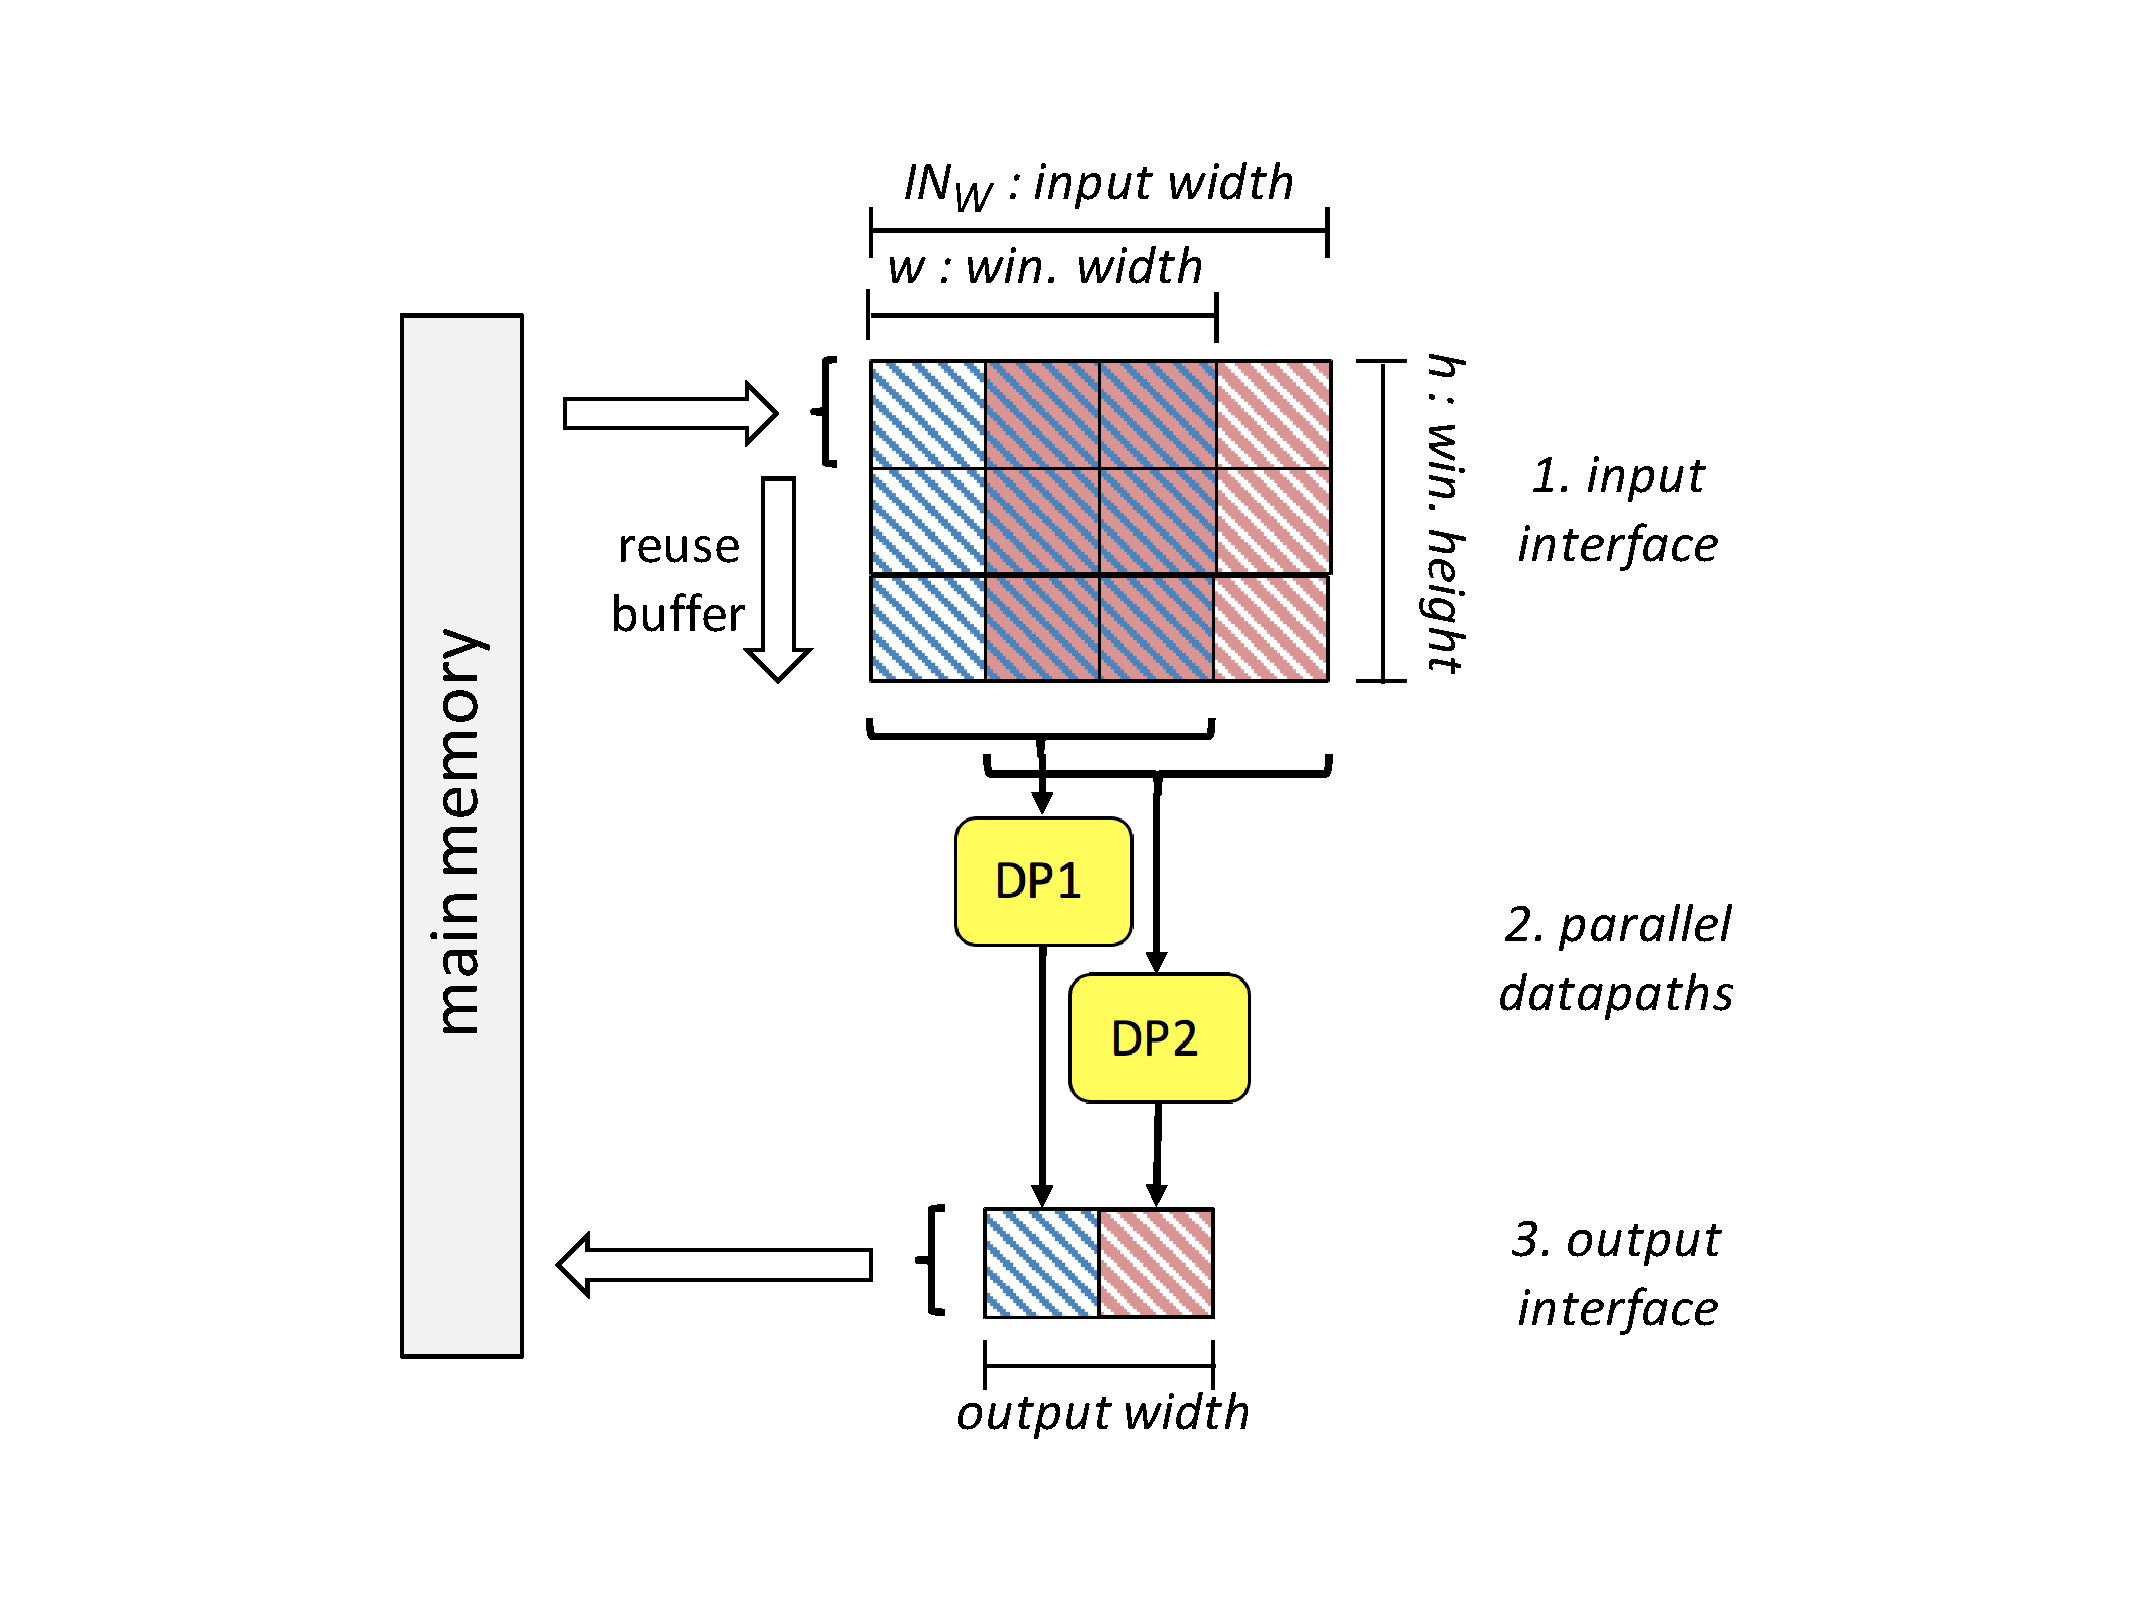
\includegraphics[width= .8 \linewidth]{figs/Data_Reuse}
\vspace*{-1cm}
\caption{Data Reuse of memory accesses (66.6\%) across consecutive iterations of a loop, in a sliding
window application.}
% \vspace*{-0.7cm}
% a figure\dots
% \caption{\textsc{Automaton} for something or other. A caption can be rather
% long and \emph{should} then consist of complete sentences ended with a `.'}
\label{fig:data_reuse}
\end{figure}


\subsubsection{Data Reuse Analysis}

In order to identify the level of data reuse that takes place throughout the execution of every
window application, there are three pieces of information that are vital: a) the size of the window, 
b) the stride and c) the frame size.
An example of data reuse, accounting for roughly 66\% the size of the window between consecutive 
iterations, can be seen in Figure \ref{fig:data_reuse}.
The window size is the access pattern
within the innermost body of the loop. The innermost and outermost
loop stride is the value of the induction variable increase for the innermost
and the outermost loop respectively. Finally, the frame size is
the iteration space within which the sliding window is moving. To extract this information 
I have developed an analysis pass, based on the LLVM Polly framework \cite{GrosserApr12}. 
Application-specific parameters are then considered in conjunction with architecture constraints 
(input/output width) to automate the synthesis of efficient HW accelerators.\par

\begin{algorithm}[t]
\begin{flushleft}
\textbf{Input:}  Application written in C/C++\\
\textbf{Output:} List of Identified SCoPs and their respective Frame, Window, Stride sizes/values.\\
\end{flushleft}
\begin{algorithmic}[1]
\Function{$RunOnRegion()$}{}
  \State\Call{$getAnalysis$}{ScopInfo}
  \State\Call{$scop=getScop()$}{}
  \State\Call{$RunOnScop$}{scop}
\EndFunction
\State
\Function{$RunOnScop$}{scop}
  \State\Call{$LI=getLoopInfo()$}{}
  \State\Call{$SE=getSE()$}{}
  \If {\Call{$L==OutermostLoop$}{}}
    \State\Call{$getTripCountFortLoop()$}{}
    \State\Call{$getStrideForLoop()$}{}
  \ElsIf  {\Call{$L==InnerMostLoop$}{}}
    \State\Call{$getReadMemoryAccesses()$}{}
    \State\Call{$ComputeDistancesForReadAccesses()$}{}
    \State\Call{$ComputeWindowSize()$}{}
  \EndIf
\EndFunction
\end{algorithmic}
\caption{LLVM Analysis Pass - SCoP Identification and 
Data Reuse Analysis}
\label{dr_Algo}
% \vspace{-0.2cm}
\end{algorithm}


The analysis pass, as seen in Algorithm  \ref{dr_Algo}, 
iterates over regions of the application 
functions and identifies Static Control Parts (SCoPs). The SCoPs are subgraphs of the control 
flow graph of a function 
where the flow of control is known statically. For each SCoP, loop and scalar evolution information
is collected from the body of the loop. \par

Loop information supports methods that can provide the 
loop depth, so as to identify the innermost loop. Scalar evolution information can be used to extract 
the loop trip count, which is the iteration space of each loop, and thus compute the frame size.
The stride value, both vertical and horizontal, is obtained by a function that was developed based
on existing methods of the Loop analysis LLVM pass.
%and receives as argument the Basic Block of the corresponding loop. 
Lastly, the read memory accesses of the innermost body of
the loop are identified by using \texttt{isl} functions, which
compute the
distance (or delta) of each of these read accesses with respect to the
first one. Given the access pattern, the window size is computed as the minimum 
enclosing rectangle. After having identified the necessary information, the implementation of a
local buffer that fits these needs can be carried out.\par

\subsubsection{Hardware Implementation}

The parameters retrieved with the analysis  pass (frame size, stride, horizontal and vertical window 
size) and the characteristics of the interconnect (input and output width) are employed to derive 
efficient HW accelerators implementation with local storage and data reuse.\par

As showcased in Figure \ref{fig:data_reuse}, accelerators implementations embed multiple 
combinatorial datapaths, each executing one iteration of the loop body of the target application.
The input interface embeds a local storage, whose horizontal size
corresponds to the available input data width of $IN_{W}$ data
elements, while its vertical size is equal to the vertical size
of the application window $h$. It is implemented as a $IN_{W} * h$
shift register, operating in the vertical (top-down) direction. During
execution, the first row of the shift register is filled with input
data in each clock cycle.  A subset of the elements stored in the
shift register is connected to each of the different datapaths
according to their managed sets, e.g.: the first one having inputs
corresponding to the buffer columns ranging from $0$ to $w - 1$ (the
horizontal size of the window) and the second one corresponding to the 
buffer columns ranging from $1$ to $w$.
Figure \ref{fig:data_reuse} illustrates such scheme for the simple case
of $IN_{W} = w+1$.\par

At the beginning of the execution, $h$ rows are stored in the shift register
before activating the datapaths logic. Afterwards, this activation is
performed for each new row, discarding the last (topmost) line and
storing a new one in the first (bottom) position of the shift
register. At the completion of a vertical slide of the window through
the frame, a new one is started, increasing the horizontal displacement 
of the buffer by $IN_{W} - w + 1$ elements.\par

Finally, since no reuse opportunities are present for outputs, 
the output interface simply concatenates the values generated by the datapaths, and
transfers them as a single and wide memory access. 

\subsection{Experimental Results}
\label{sec:dr_exp}

The evaluation of this approach is carried out in three benchmarks of varying window sizes.
\texttt{Sobel} is an edge detection algorithm with an access pattern of a 3x3 window. \texttt{BlockSAD} 
is a kernel in \htsf and is used to detect the similarity among 4x4 blocks. Finally, 
\texttt{Maximum Filter} computes the brightest pixel among neighbors in 8x8 blocks. Three different 
configurations were considered, spanning from a singe datapath and minimum input width (Conf.1) 
to multiple datapaths and increased input width (Conf.2 and Conf.3) as seen in Figure \ref{fig:data_reuse}. 
Multiple datapaths translate to 
more parallel windows executing and, hence, increased demand in area resources.\par

The comparison of the approach introduced above is carried out against two state-of-the-art HLS 
tools: ROCCC and Vivado\_HLS. Vivado\_HLS is compared in two modes, one being the default and
the other one after extensive manual rewrite of the source code in order to obtain increased data 
reuse.

\begin{figure}[h!]
\centering
\hspace*{-2cm}
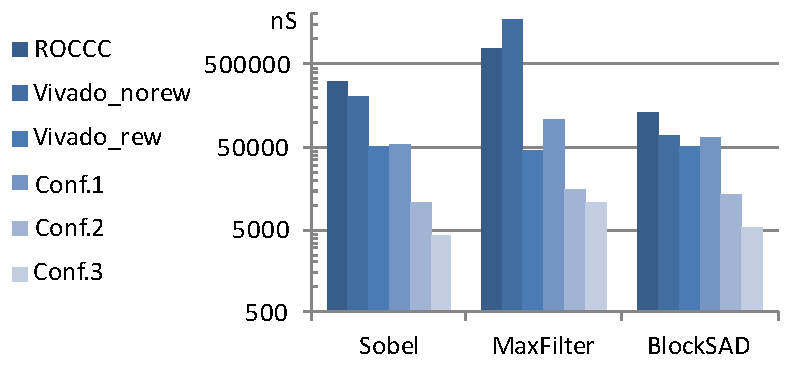
\includegraphics[width= .7 \linewidth]{figs/exec_time_fpga}
\caption{Execution time to process a 100x100 frame.}
\label{fig:exec_time_fpga}
\end{figure}

\begin{figure}[h!]
\centering
\hspace*{-1cm}
\vspace{1cm}
\vskip -1em 
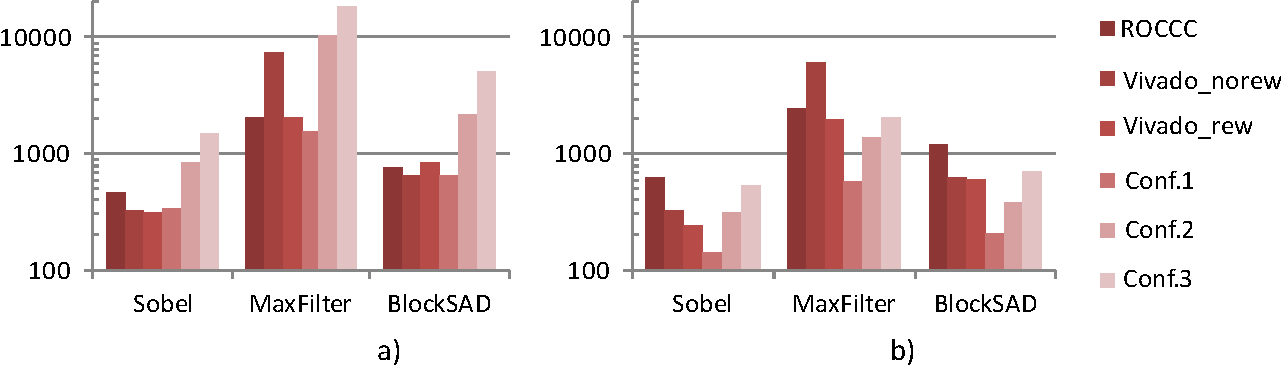
\includegraphics[width= 1 \textwidth]{figs/area_fpga}
\caption{Comparison of required resources for our generated systems and for baseline 
approaches: LUTs (a) and Flip-Flops (b).}
\label{fig:area_fpga}
\end{figure}

Execution time, as seen in Figure \ref{fig:exec_time_fpga}, is extracted from 
a targeted Xilinx Virtex7 FPGA platform. 
It can be observed that ROCCC systems have similar
performance with respect to Vivado\_norew ones. Conf.1 accelerators 
--- even though they do not require code modifications --- are as 
efficient as Vivado\_rew ones. Conf.2 and Conf. 3 that are
supported only by the framework presented in \ref{sec:dr_meth}, dramatically decrease
run-times, with an order-of-magnitude speed up on average between
Conf.1 and Conf.3. The other state of the art tools \emph{fail to 
provide an equivalent solution with such low execution time}.
Figure \ref{fig:area_fpga} reports the amount of area resources required by
ROCCC, Vivado\_HLS and our own generated accelerators.
Unsurprisingly, accelerators featuring a high number of datapaths (Conf.3) 
require more resources than single-datapaths approaches (Conf.1, Vivado). 
Nevertheless, the area increase in terms of Flip-Flops is comparable to 
the other to state-of-the-art tools, as the size of the buffer only is 
increased slightly to support a high degree of parallelism.
On the other hand, the results highlight that complex accelerators require 
an increased amount of combinatorial logic (LUTs), with respect to ROCCC 
and Vivado\_HLS.

\vspace{-0.3cm}
\subsection{Conclusions}

It has been demonstrated that static source code analysis can be crucial, when it comes to 
automatically optimizing the synthesis of accelerators that are dedicated to 
sliding window applications. My SW analysis identifies data reuse, as well as data locality,
and subsequently allows to exploit these characteristics by making use of appropriate
memory buffers. The experimental results reveal an order-of-magnitude performance 
improvement with respect to \SoTA\ methodologies. This work was published in 
HiPEAC IMPACT 2017 Seventh International Workshop on Polyhedral Compilation Techniques 
\cite{ZacharopoulosJan17}. 

% SECTION 2.2
%

\section[Machine Learning Approach for Loop Unrolling\\ Factor Prediction]
{Machine Learning Approach for Loop Unrolling\\ Factor Prediction}

\subsection{Motivation}

\HLS\ tools, utilized to synthesize accelerators, require manual decisions to be made, so as 
to build efficient accelerators. These decisions regard the choice of high-level optimizations 
and transformations to be applied, therefore a good understanding of the SW parts to be 
accelerated is essential. Optimizations applied during synthesis can highly improve the performance 
achieved, as well as allocate less HW resources for a given computer architecture. Nonetheless, 
the selection of optimizations is a challenging task due to two main reasons. 
First, hardware synthesis is a time-consuming process, limiting in practice the amount of 
possible implementations that can be evaluated. Second, the effect of assigning different values to 
directives is difficult to foresee, due to low-level application characteristics.\par

Simulation tools such as Aladdin \cite{ShaoJul14} have been developed in order to rapidly 
estimate the performance and cost (area) of HLS-defined designs. Nonetheless, even when employing 
estimation tools, an exhaustive evaluation of all directives settings for each candidate accelerator 
in a heterogeneous system is still unfeasible beyond simple cases. Addressing
this challenge, a machine learning framework is proposed that is able to infer the proper 
implementation of an HLS design based on its characteristics, automatically derived from a source code 
analysis pass, based within the LLVM compiler framework \cite{LattnerMar04}.\par


Within the scope of this piece of research, the focus is placed on {\em loop unrolling}, an already 
well known optimization from the compiler domain, as well as the HW domain.
The loop unrolling optimization replicates the body of a loop a given number of times 
in order to expose parallelism, which especially in a HW implementation can lead to 
substantial speedup gains \cite{KurraApr07}. 
% On the other hand this might raise the need for more HW resources. 
This directive should nonetheless be applied sensibly, because it entails a high area cost for the 
duplicated logic; in addition, its ensuing benefits can be hampered by loop-carried dependencies 
and frequent memory accesses.\par

It is thus clear that there is a trade-off between execution time and the area budget that 
a computer architect has at hand, as well as the level of complexity and more potential 
side effects that need to be taken into consideration. Since HW realizations are targeted, 
the goal of this work is to reach a {\em sweet spot} between performance and HW resources.\par

Within the sphere of this research work, the following contributions are made.
First, a novel {\em \ML\ }
approach is introduced, based on Random Forest classification, 
instead of estimation-based models, to predict 
accurately the optimal loop unrolling factor of loops in applications to be synthesized
in HW. The use of this methodology can provide results with better prediction score
and in much less time, compared to the \SoTA.
Second, the whole process is fully automated, from the analysis of the input applications, 
using the LLVM compiler infrastructure \cite{LattnerMar04}, up to the training of the Random 
Forest Classifier. Finally, the trained \RF\ classifier can be used to generate accurate loop 
unrolling predictions for any given application -- a piece of information that can 
directly be used by an HLS tool such as Vivado\_HLS, in order to synthesize parts of these 
applications to HW.

\subsection{Related Work}

Research papers have explored the applicability of machine learning to apply
compiler optimizations. In \SW\ compilers, it has been
employed by Agakov et al. \cite{AgakovMar06} to speed up iterative compilation,
by Monsifrot et al. \cite{MonsifrotAug02} to produce compiler heuristics
and by Kulkarni et al. \cite{KulkarniOct12} to select the order in which optimization passes
should be performed. Stephenson et al. \cite{StephensonApr05} have made use of Supervised 
Classification, such as near neighbor (NN) classification 
and Support Vector Machines (SVM) methods, to produce accurate predictions in optimal unrolling 
factors.
In all above-mentioned research works the authors targeted \SW\ 
compilation; in Subsection \ref{sec:ml_exp}, a comparative performance evaluation of the 
framework presented in Subsection \ref{sec:ml_meth} to the methodology proposed by 
Stephenson et al. is carried out, showcasing the benefit of the choice of loop features and 
classification strategy in the HLS scenario.\par

Liu et al.  \cite{LiuJun13} used a \RF\
classification model in the context of HLS, extending the \ItRef\
framework proposed in \cite{MarianiApr12} \cite{PalermoNov09}
\cite{XydisMar13} and \cite{ZuluagaJun12}. They address a different
problem with respect to the one tackled in this section: that of retrieving the set of
Pareto-optimal implementations of a given design by navigating its
configuration space. A similar stance, addressing system-level design,
is illustrated by Ozisikyilmaz et al. \cite{OzisikyilmazJun08}.  As
opposed to these works, my aim is to perform a predictive assignment
of synthesis directives, based on a training performed on an independent
input set. This problem was also investigated by Kurra et
al. \cite{KurraApr07}. Contrary to their methodology, my methodology does not
depend on a detailed estimation delay model of the loop body so as to
predict loop unrolling factors in HLS instances.

\begin{figure}[h!]
\centering
% \hspace*{-2cm}
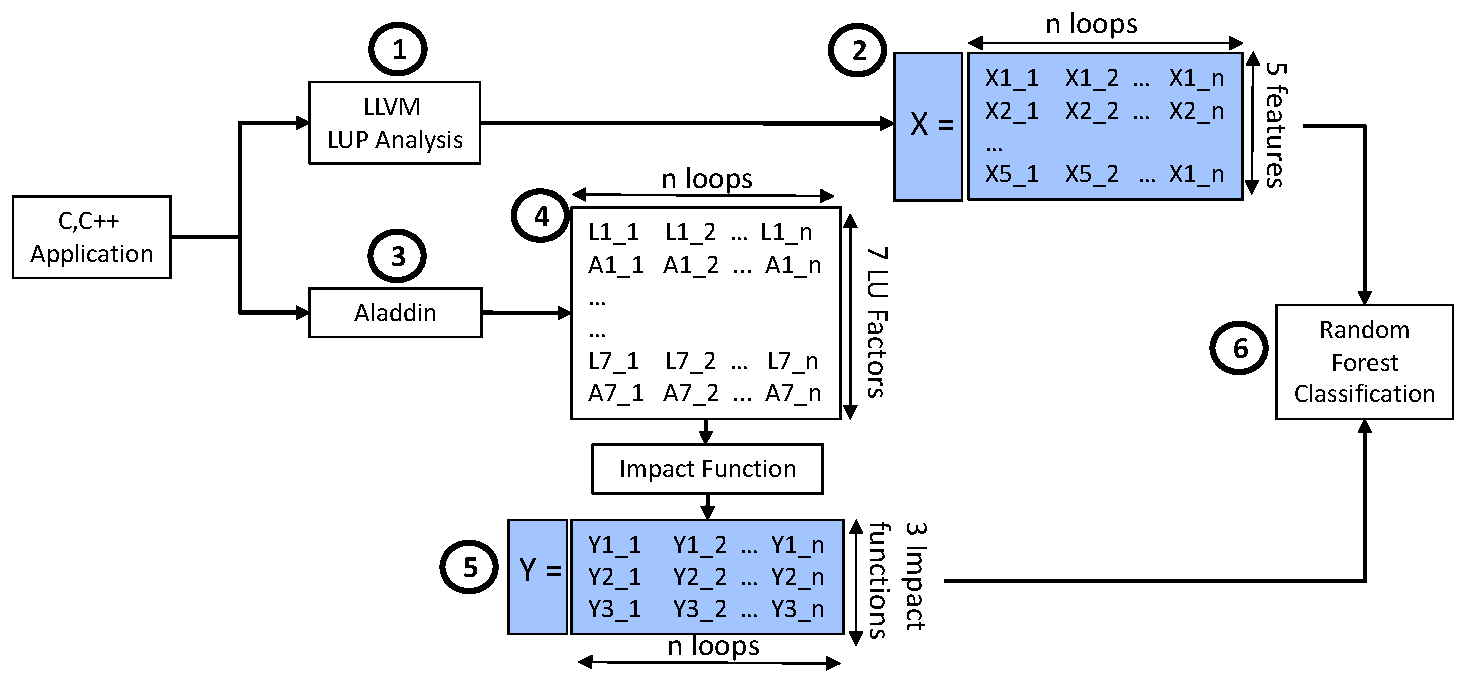
\includegraphics[width= 1 \linewidth]{figs/LUP_method}
\caption{Overview of the Loop Unrolling Prediction methodology.}
\label{fig:lup_method}
\end{figure}

\subsection{Methodology}
\label{sec:ml_meth}

In this section, first the employed objective function that determines the optimal loop 
unrolling factor is presented.
% , as well as the performance metrics considered to evaluate 
% the framework performance. 
Then, the LLVM analysis pass that was developed in order to 
automatically extract relevant loop features and the approach followed to retrieve the 
area and run-time performance of HLS designs is detailed. Lastly, the supervised learning 
classifier method is demonstrated, which, during the training phase, gathers the data from the 
previous steps to produce a loop unrolling predictor, and, during the test phases, assigns 
loop unrolling factors based on loop features.\par

\subsubsection{Optimal Loop Unrolling Factor -- Objective Function}

The {\em optimal loop unrolling factor} is defined as follows.
Given a defined set of unrolling factors S: <1, 2, 4, 8, 16, 32, 64>, there is one for every
loop that maximizes the \textbf {Impact (I)}, given by the following formula:

$$I(L,A)= \alpha  \cdot \dfrac{ (L_1 - L)} {L_1} + \beta \cdot \dfrac{ (A_1 - A)} {A_1},\ \alpha + \beta = 1$$

Where $L_1$ is the latency of the of the function containing a loop and being synthesized as HW 
accelerator, for Loop Unrolling Factor (LUF) that is equal to one, i.e., a fully rolled loop. $L$ 
is the latency of the HW accelerator for any possible LUF from the defined set.
Respectively, $A_1$ is the area resources requirements of the HW accelerator with LUF equal to one and 
$A$ the area for any possible LUF from the defined set.\par

Subsequently, the optimal LUF is defined as the one that maximizes the Impact function above. Note that, 
when $LUF = 1$, then $I(L,A)=0$ which corresponds to a baseline implementation. $I(L,A)$ may also 
be negative for suboptimal LUF choices (where unrolling might increase area without decreasing 
latency), but will always be $\ge 0$ for optimal unrolling factors.\par


For the evaluation presented in Subsection \ref{sec:ml_exp}
three different strategies were considered: a) Optimize for both latency and area ($\alpha = 
\beta = 0.5$). In this configuration a balance is maintained between decreasing the number of 
execution cycles and keeping low the usage of HW area resources in a given implementation.
b) Optimize for latency ($\alpha = 0.7, \beta = 0.3$). Minimizing latency is favored by this
approach, thus focusing on increasing the speedup of an application, and finally c) Optimize
for area ($\alpha = 0.3, \beta = 0.7$). This approach aims at decreasing the area budget of 
the implementation, therefore achieving an average speedup, but maintain low usage of HW 
area resources. All three configurations fulfill different architectural needs and explore 
realistic alternative scenarios.\par

% To evaluate the classification performance of a trained classifier, two different metrics were
% adopted. The \emph{Prediction Score} states the
% percentage of optimal (according to $I(L,A)$ ) LUFs that were correctly
% identified on the out-of-sample test set. The \emph{Average Error}
% instead measures the average distance between the indexes in $S$ of the
% correct and the predicted LUF.


\subsubsection{LLVM Analysis Pass -- Loop Features Extraction}

Loop features are automatically identified by an analysis pass (depicted as 
point 1 in Figure~\ref{fig:lup_method}) that was developed within the LLVM 
compiler infrastructure \cite{LattnerMar04}. Features are retrieved starting from
applications written in C or C++, operating on their Intermediate
Representation, provided by the LLVM front-end passes.\par  

My \textit{LLVM Loop Unrolling Prediction Analysis Pass} iterates over functions
of the applications and identifies loops. On each of them, it performs
loop, scalar evolution and dependence analysis to extract their
features, summarized in Table \ref{tab:X}: the critical path, the trip
count, the presence of loop carried dependencies and the required
memory accesses (load and stores).\par

% Table 1 and 2
%
%
\begin{table}[h]
  \centering

  \small\addtolength{\tabcolsep}{-3pt}
  \vspace{1em}
  \begin{tabular}{| l |} 
 \hline    
 \textbf{Features - X Vector}  \\ \hline
    \emph{Critical Path}      \\ \hline
   \emph{ Loop\ Trip\ Count} \\ \hline
   \emph{ Has\ Loop\ Carried\ Dependencies}     \\ \hline
   \emph{ \#\ Load\ Instructions}     \\ \hline
   \emph{ \#\ Store\ Instructions}      \\ \hline
  \end{tabular} 
    \caption{Features extracted by LLVM LU Analysis Pass.}
      \label{tab:X}
  
  
     \vspace{2em}
  

  \begin{tabular}{| l | l |} 
 \hline    
 \textbf{Features - X Vector 1} & \textbf{Features - X Vector 2}  \\ \hline
  \emph{\#\ Operands}        &\emph{\#\ Floating\ Point\ Operations}        \\ \hline
  \emph{Range\ Size}     &\emph{Loop\ Nest\ Level}   \\ \hline
    \emph{Critical\ Path}   &\emph{\#\ Operands}  \\ \hline
  \emph{\#\ Operations}      &\emph{\#\ Branches}   \\ \hline
  \emph{Loop\ Trip\ Count}&\emph{\#\ Memory\ Operations}   \\ \hline
  \end{tabular}
    \caption{Feature vectors selected by Stephenson et al. \cite{StephensonApr05}.}
      \label{tab:St_X1_X2}
\end{table}

The choice of features is based on the factors that influence the cost
and the achievable speedup of \HW\ unrolled loops: a loop with a
long critical path may be expensive to duplicate, while loop carried
dependencies and memory accesses may force a serialization of
execution irrespectively of the degree of unrolling. These
considerations lead us to consider a markedly different feature list
with respect to works focusing on software targets, such as the one of
Stephenson et al. (Table \ref{tab:St_X1_X2}).\par

\begin{algorithm}[t]
\begin{flushleft}
\textbf{Input:}  Application written in C, C++\\
\textbf{Output:} X (Feature Vector)\\
\end{flushleft}
\begin{algorithmic}[1]
\Function{\emph{RunOnFunction}} { }
  \For {\emph{BB\ in\ Function} }
    \If {{\emph{L=getLoopForBB}() } } {}
      \State{\emph{LoopUnrollingPredictionAnalysis}}{(BB,L)}
    \EndIf
  \EndFor
\EndFunction
\State
\Function{\emph{LoopUnrollingPredictionAnalysis}}{Basic Block BB, Loop L}
  \State{\emph{ LI=getLoopInfoAnalysis}()}
  \State{\emph{SE=getScalarEvolutionAnalysis()} } {}
  \State{\emph{DA=getDependenceAnalysis()}} {}
  \State{\emph{/*\ Gather\ Features\ for\ X\ Vector */} }
  \State{\emph{x1=getCriticalPath}}{(BB)}
  \State{\emph{x2=getTripCountForLoop}}{(L)}
  \State{\emph{x3=getLoopCarriedDependencies}}{(BB)}
  \State{\emph{x4=getNumberOfLoadInstructions}}{(BB)}
  \State{\emph{x5=getNumberOfStoreInstructions}}{(BB)}
\EndFunction
\end{algorithmic}
\caption{LLVM Analysis Pass - Loop Unrolling Prediction Analysis} 
\label{Algo_LLVM}

\end{algorithm}

\subsubsection{Latency and Area Estimation}
\label{sec:ml_la}

To establish a link between LUFs and performance/cost of
implementations, latency and area values must be extracted both for
the loops in the training set (in order to optimize the classifier)
and the ones in the test set (to measure its accuracy).%\par
Aladdin \cite{ShaoJul14} (point 3 in
Figure~\ref{fig:lup_method}), a pre-RTL power-performance simulator
for \HW\ accelerators was utilized in order to retrieve latency and area 
information. All functions in the considered benchmarks were
simulated by employing each feasible unrolling factor in the $S$ set 
defined above on every loop contained.  
Latency is reported by Aladdin in clock cycles,
while area is expressed in $\mu m^2$ in a $45nm$ technology. The
result is shown as point 4 in Figure~\ref{fig:lup_method}.
\par

The Impact ($I$) was computed afterwards for the different $\alpha$
and $\beta$ values, to retrieve the optimal loop unrolling factor for every loop
of a function, which is the index of the LUF that maximizes $I$. The
result is three vectors $\{Y1,Y2,Y3\}$ (point 5 in
Figure~\ref{fig:lup_method}) that contain the target values for the
classification algorithm. The $Y1$ vector includes the optimal loop
unrolling factor that balances the \HW\ implementation of the
accelerators in terms of low latency and low area. Values in the $Y2$
vector favors low-latency implementations, applying more aggressive
loop unrolling, whereas $Y3$ favors low-area ones.


\subsubsection{Random Forest Classification}


This information (X and Y vectors) extracted as described above are used 
as input to a Random Forest (RF) classifier (point 6 in
Figure~\ref{fig:lup_method}).
Supervised learning is performed by detecting the correlation between 
the input, the compiler extracted information, used as the X feature vector, 
and the output, which is the optimal loop unrolling factor for each loop.\par

\RF\ was used as the supervised learning model, which has been shown by Liu et al.
\cite{LiuJun13} to outperform alternatives such as Multilayer Neural Networks and \SVM\  
classification in the context of HLS design space exploration. \RF\ algorithms follow
a decision tree methodology, combining many weak classifiers to derive a strong one, allowing
the generation of low-complexity and robust classifiers.\par

\begin{algorithm}[t]
\begin{flushleft}
\textbf{Input:}  X and Y Vectors\\
\textbf{Output:} Trained Random Forest Classifier\\
\end{flushleft}
\begin{algorithmic}[1]
%\State{$NumberOfTrainingSessions=1000$}
\For {\emph{ i\ in\ NumberOfTrainingSessions} }
  \State{\emph{ X\_train, X\_test, Y\_train, Y\_test=train\_test\_split(X,Y)} }
  \State{\emph{ /*\ Training\ Phase\ */} }
  \State{\emph{ M=RandomForestLearningModel} }
  \State{\emph{ M.train(X\_train, Y\_train)} }
  \State{\emph{ /*\ Evaluation\ Phase\ */} }
  \State{\emph{ Pred=M.predict(X\_test)} }
  \State{\emph{ Error=abs(Pred-Y\_test)} }
  \State{\emph{ Score=M.score(X\_test-Y\_test)} }
\EndFor
\end{algorithmic}
\caption{Random Forest Classification -
 Training and Test} 
 \label{algo:RF}
\end{algorithm}

The algorithm employed, as presented in Algorithm \ref{algo:RF},
follows an approach similar to a \textit{k-fold cross validation}
strategy.  The whole data set ($X$ and $Y$ vectors, see points 2 and 5 
in Figure \ref{fig:lup_method}) is divided randomly
between a training set and a test set, where the training set is equal
to 80\% of the whole data set and the remaining 20\% is the test set.
Then, the \RF\ model is used for the training process on the training
set and out-of-sample predictions are carried out for each element of
the test set. After all predictions on the test set have been
computed, the prediction score and the average error (as defined in
Subsection \ref{sec:ml_exp}) are computed for the current training
session.\par

\subsection{Experimental Results}
\label{sec:ml_exp}

To evaluate the classification performance of a trained classifier, two different metrics were
adopted. The \emph{Prediction Score} states the
percentage of optimal (according to $I(L,A)$ ) LUFs that were correctly
identified on the out-of-sample test set. The \emph{Average Error}
instead measures the average distance between the indexes in $S$ of the
correct and the predicted LUF.\par

In order to comparatively evaluate the proposed methodology, combining \RF\ classification and
LLVM-based loop features extraction, benchmarks of different complexity were considered. Small 
and medium-sized ones are \adpcm, an audio encoding kernel, \stencil, an 
implementation of an iterative algorithm that updates array elements according to a given pattern, 
and \sha, a secure hash encryption method
used in the information security domain. \jpeg\ and \mpeg\ are instead larger benchmarks, which 
perform image and video compression, respectively.
Applications were drawn from the CHStone  \cite{HaraMay08} and the Scalable Heterogeneous 
Computing (SHOC) benchmark suites \cite{DanalisMar10}. In total, they comprise 87 different loops.\par

% The benchmarks used during the experimental phase are broadly used embedded applications from 
% the CHStone suite \cite{HaraMay08} and SHOC suite \cite{danalis2010scalable}.
%  \adpcm, \jpeg, \mpeg, \sha\ and \stencil.\par

Random Forest classification was implemented using the Scikit-learn suite \cite{PedregosaOct11}, 
that includes \SoTA\ implementations of \ML\ models in python. Scikit-learn was also employed to 
re-implement the two methods proposed by Stephenson et al. \cite{StephensonApr05}, that are consider 
as baselines.\par

Giving an initial proof of concept for the strategy proposed, Figure \ref{fig:dist} reports the 
difference between the indexes of the predicted optimal (according to impact value) loop unrolling 
factors and the ones retrieved with an exhaustive exploration, considering 18.000 out-of-sample 
predictions on all the benchmark loops. Results are highly concentrated on zero, 
indicating a high rate of correct predictions.\par

\begin{figure}[h]
\centering
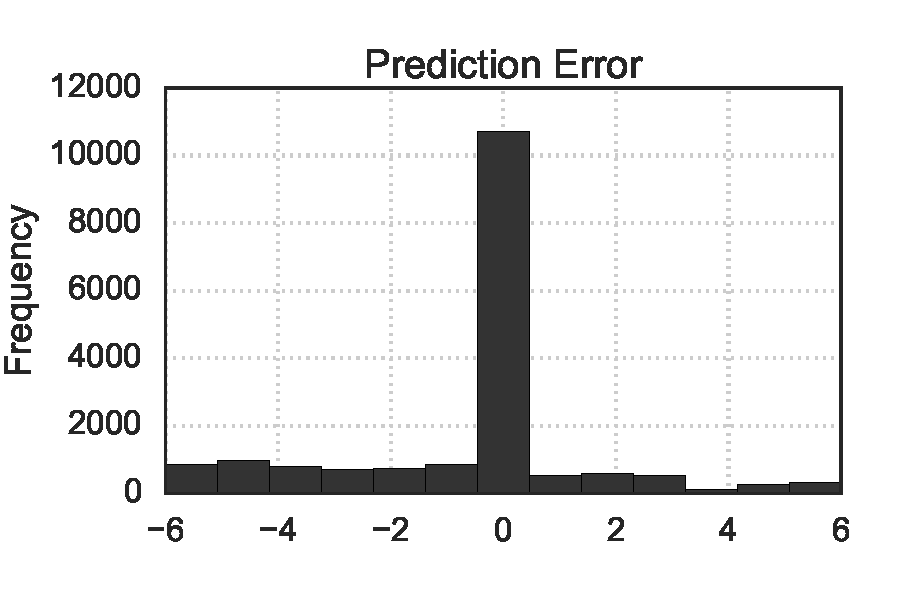
\includegraphics[width=.5\linewidth]{figs/prediction_errors}
\vspace{-1em}
\caption{Distribution of Loop Unrolling Factor Prediction Errors over 18.000 
out-of-sample predictions.}
\label{fig:dist}

\end{figure}

% During the experimental phase, state-of-the-art machine learning algorithms were used from the 
% Scikit-learn framework \cite{pedregosa2011scikit}.
% %  A Random Forest (RF) Classifier model is employed
% % to perform the classification. Results showcased a 60\% prediction absolute accuracy, meaning that the
% % predictions performed on the unknown subset of loops were correct 60\% of the time.
% As seen in Figure \ref{fig:mod_score} Random Forest (RF) is compared to Near Neighbor(NN) and
% Support Vector Machine (SVM) classifiers, and across different feature vectors. X as described
% above and X1,X2 by \cite{StephensonApr05}. The X1 and X2 features differ from the ones of X (e.g. X2: \# 
% Floating Point operations, loop nest level etc) as they target 
% SW execution. The suggested RF classifier and X feature vector 
% showcased a 60\% prediction absolute accuracy, meaning that the predictions performed on the unknown 
% subset of loops were correct 60\% of the time, outperforming every other state-of-the-art approach.

\subsubsection{Classification Models and Features}
\label{subsec:mode_feature}

The evaluation of the choice of features ($X$ vector in Table \ref{tab:X}) and training model \RF\ 
(RF), takes place against two \SoTA\ methodologies proposed by Stephenson et al. 
\cite{StephensonApr05}. The latter present different classification strategies: 
\SVM\ (SVM) and \NN\ (NN) and a different choice of investigated loop features, reported in 
Table \ref{tab:St_X1_X2}. Figure \ref{fig:mod_score} shows, for a choice of $\alpha = 0.5$, the 
prediction score and the average error of the nine strategies resulting from different feature 
vectors and classification strategies. Experimental results highlight that the presented framework 
($X$ feature vector and RF classification)
outperform other choices, reaching a prediction score above  60\% and an average error of
less than 1.4. Similar results were obtained for impact functions favoring area or latency
($Y2$ and $Y3$ vectors).



\begin{figure*}

\centering
%\hspace*{-2cm}
%\vspace{-0.4cm}
  \hspace*{-2cm}
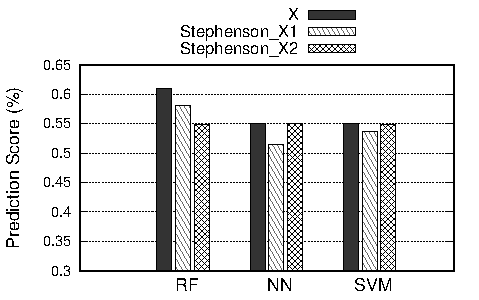
\includegraphics[width= .5 \linewidth]{figs/models_score}
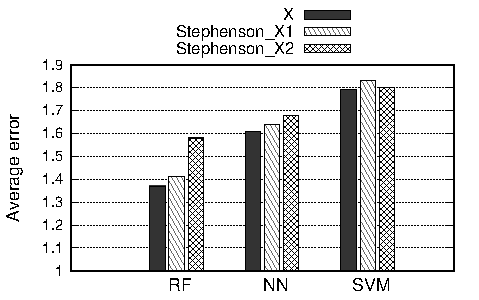
\includegraphics[width= .5 \linewidth]{figs/models_error}
% \vspace*{-0.2cm}
\hspace*{-2cm}
\vspace*{-0.2cm}
\caption{Left: Comparison of the Prediction Score across Random Forest, Nearest Neighbor, Support Vector Machines models 
and the respective feature selection: X vector, Stephenson et al. X1 and X2 vectors \cite{StephensonApr05}.
Right: Features extracted by my LLVM Loop Unrolling Analysis Pass.}
\label{fig:mod_score}
% \vspace*{-0.7cm}
\end{figure*}




\subsubsection{Iterative Refinement}

In the second round of experiments, the comparison of the proposed method was carried out against an 
\ItRef\ approach, used in \cite{MarianiApr12} \cite{PalermoNov09} \cite{XydisMar13} \cite{ZuluagaJun12}. 
\ItRef\ uses part of the training data set
to obtain a first version of the classifier, whose performance is then improved by using a second,
disjoint set of input and outputs.\par

For this evaluation, three different settings of Y target vectors $\{Y1,Y2,Y3\}$ were considered, as 
described in Subsection \ref{sec:ml_la}. The employed data,
the features ($X$ vector) and the training model (\RF) were the same both for Algorithm \ref{algo:RF} 
and the one using \ItRef. For \ItRef, 75\% of the training set is allocated for the 
initial training phase, and the remaining 25\% for the refinement phase.

\begin{figure*}
\centering
%\hspace*{-2cm}
%\vspace{-0.4cm}
  \hspace*{-2cm}
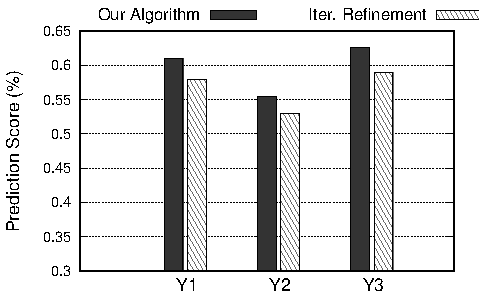
\includegraphics[width= .5 \linewidth]{figs/iter_ref_score}
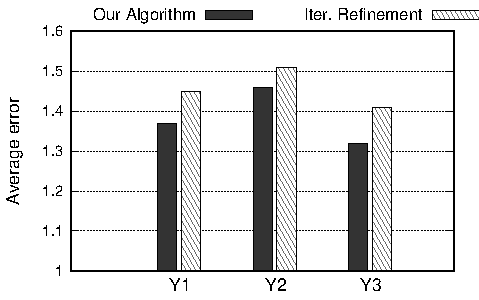
\includegraphics[width= .5 \linewidth]{figs/iter_ref_error}
% \vspace*{-0.2cm}
\hspace*{-2cm}
\vspace*{-0.2cm}
\caption{Left: Comparison of the Prediction Score across Random Forest, Nearest Neighbor, Support Vector Machines models 
and the respective feature selection: X vector, Stephenson et al. X1 and X2 vectors \cite{StephensonApr05}.
Right: Features extracted by my LLVM Loop Unrolling Analysis Pass.}
\label{fig:iter_ref_score}
% \vspace*{-0.7cm}
\end{figure*}

The prediction score, as seen in Figure \ref{fig:iter_ref_score}, ranges from 53\% to 63\% across the three 
$Y$ vectors. Nevertheless, our methodology consistently outperforms the \ItRef\ approach, while achieving 
the highest prediction score (63\%) for the setting that favors low area resources ($Y3$). A similar
observation can be made for the average error values, where the suggested approach keeps a lower 
average error for all predictions, across all vectors, with the one related to the $Y3$ vector 
being the lowest (1.32).\par

\subsection{Conclusions}

A novel methodology based on LLVM analysis and Random Forest classification that performs loop unrolling 
factor prediction for HLS designs was performed. This approach achieves better prediction score 
in comparison to state-of-the-art Machine Learning methods. Experimental evidence showcases that, 
by carrying out accurate predictions of loop unrolling factors, high performance accelerator 
implementations can be realized, while avoiding time-consuming exhaustive explorations. This work was 
published in the 2018 International Conference on High Performance Computing \& Simulation (HPCS) 
\cite{ZacharopoulosJul18}.


%
%
%
%
%  
%     CHAPTER 3
%
%
%
%
%


\chapter[System Aware Accelerators Identification]
{System Aware Accelerators Identification}
% {System Aware Accelerators Identification --- Speedup and Energy Efficiency}

In the final Chapter of the dissertation the notion of automatic selection of HW accelerators is extended
by taking into account the underlying system where the specialized accelerators are hosted. The knowledge
of the characteristics of the system that is targeted can be critical for the choice of the HW accelerators
to be implemented. The memory system of a platform for instance can vastly affect the latency due to data
exchange between the main memory of the system and the HW accelerators. 
\aseeker, an LLVM-based tool-chain, is presented as a framework that performs automatic identification 
and selection of HW accelerators targeted to a specific \SoC\ (SoC).
\aseeker\ performs thorough analysis of applications source code and estimates memory latency along with 
computational latency of candidates for acceleration. The granularity of the candidates for acceleration 
is expanded to that of a subgraph of the entire call graph of an application to accommodate for the 
communication overhead between main memory and the HW accelerators. 
\textbf{NOTE:} Write for EnergySeeker.

\section{\aseeker: Accelerators for Speedup}

\subsection{Motivation}

System-level design, and heterogeneous computing as a whole, is witnessing a breakthrough. 
Emerging best practices based on High Level Synthesis (HLS) allow unprecedented productivity levels. 
HLS dramatically shortens development cycles by employing C/C++ descriptions as entry points 
for the development of both \SW\ (SW) and \HW\ (HW) greatly facilitating the task of migrating 
functionalities between the two.\par

However, the design of heterogeneous systems comprising SW processors and HW accelerators is still a 
demanding endeavor, during which key decisions are left solely to manual effort and designer expertise 
\cite{CacciottiSep18} \cite{NouriJun17}. Furthermore, the long time required for HW synthesis, coupled 
with the huge space of alternative implementations exposed by real-world applications, limits in practice 
the number of accelerator choices that can be considered manually by a designer before HW/SW partitioning 
is settled.\par

In order to limit the entailed design effort, it is therefore crucial to identify the set of viable 
acceleration options quickly, and also early in the design process, before performing later and more 
detailed estimations. This key step is currently poorly supported by design automation tools. Indeed, 
\SoTA\ early partitioning strategies are solely based on profiling information \cite{XilinxESTRef18} 
\cite{LattnerMar04} which, as was also shown by the authors of \cite{SyrowikJun18}, may often be 
misleading.\par

To fill this gap and offer an efficient solution to the problem stated above, \aseeker is presented. 
\aseeker\ offers a methodology to identify and select the suitable acceleration candidates in an
application, from its software source code. Being implemented within the LLVM \cite{LattnerMar04} compiler 
infrastructure, first models an estimation of the cost (required resources) and merit (potential speedup) 
of all candidate accelerators in a single, quick pass, and then selects the set that maximizes the estimated 
speedup, while not exceeding a resource target. The use of \aseeker\ can therefore guide Integrated Circuit 
architects in the early design phases, highlighting which segments of a computing flow should be
targeted with HLS, and hence where to focus the process of applying optimizations to.\par

On the other hand, it indicates which parts are not likely to yield tangible benefits if realized in HW --- either 
because they present a low computational footprint, or because their characteristics hamper their potential for HW 
acceleration, e.g. they require an excessive amount of data transfers while performing limited computations.\par

The approach of \aseeker\ is markedly different from that of performance estimators, as the most promising candidates 
are identified in a single, high-level exploration, reducing the scope of further, and more detailed, estimations. It 
also differs from approaches based solely on profiling information, as profilers do not offer a measure of costs and 
run-times of HW implementations. Furthermore, they do not account for invocation overheads -- potentially leading to the 
selection of frequently called, but small, candidates. Finally, data transfers is an important factor that \SoTA\ profilers
do not take into account -- hence potentially suggesting candidates requiring an excessive amount of communication, that in 
turn can significantly weaken any potential performance gained. \aseeker, instead, takes into account both the communication 
overhead and all the characteristics of the platform that are required in order to generate an estimation model which leads
to high-performance HW accelerators choices.

\subsection{Related Work}

High Level Synthesis tools have considerably matured in recent years \cite{MeeusSep12}. Nowadays, available 
commercial tools (e.g.: Xilinx Vivado HLS \cite{VivadoHLSMar17}, Cadence Stratus HLS \cite{StratusHLSApr16}), 
as well as academic alternatives (e.g.: Legup \cite{CanisSep13}, Bambu \cite{PilatoMar12}) support the design 
of very large accelerators from C/C++ code. They reach performance levels comparable to hand-crafted 
implementations specified in low-level Hardware Description Languages (HDL) such as VHDL or Verilog 
\cite{LiuFeb16}.\par

\begin{figure}[!t]
  
  \centering
  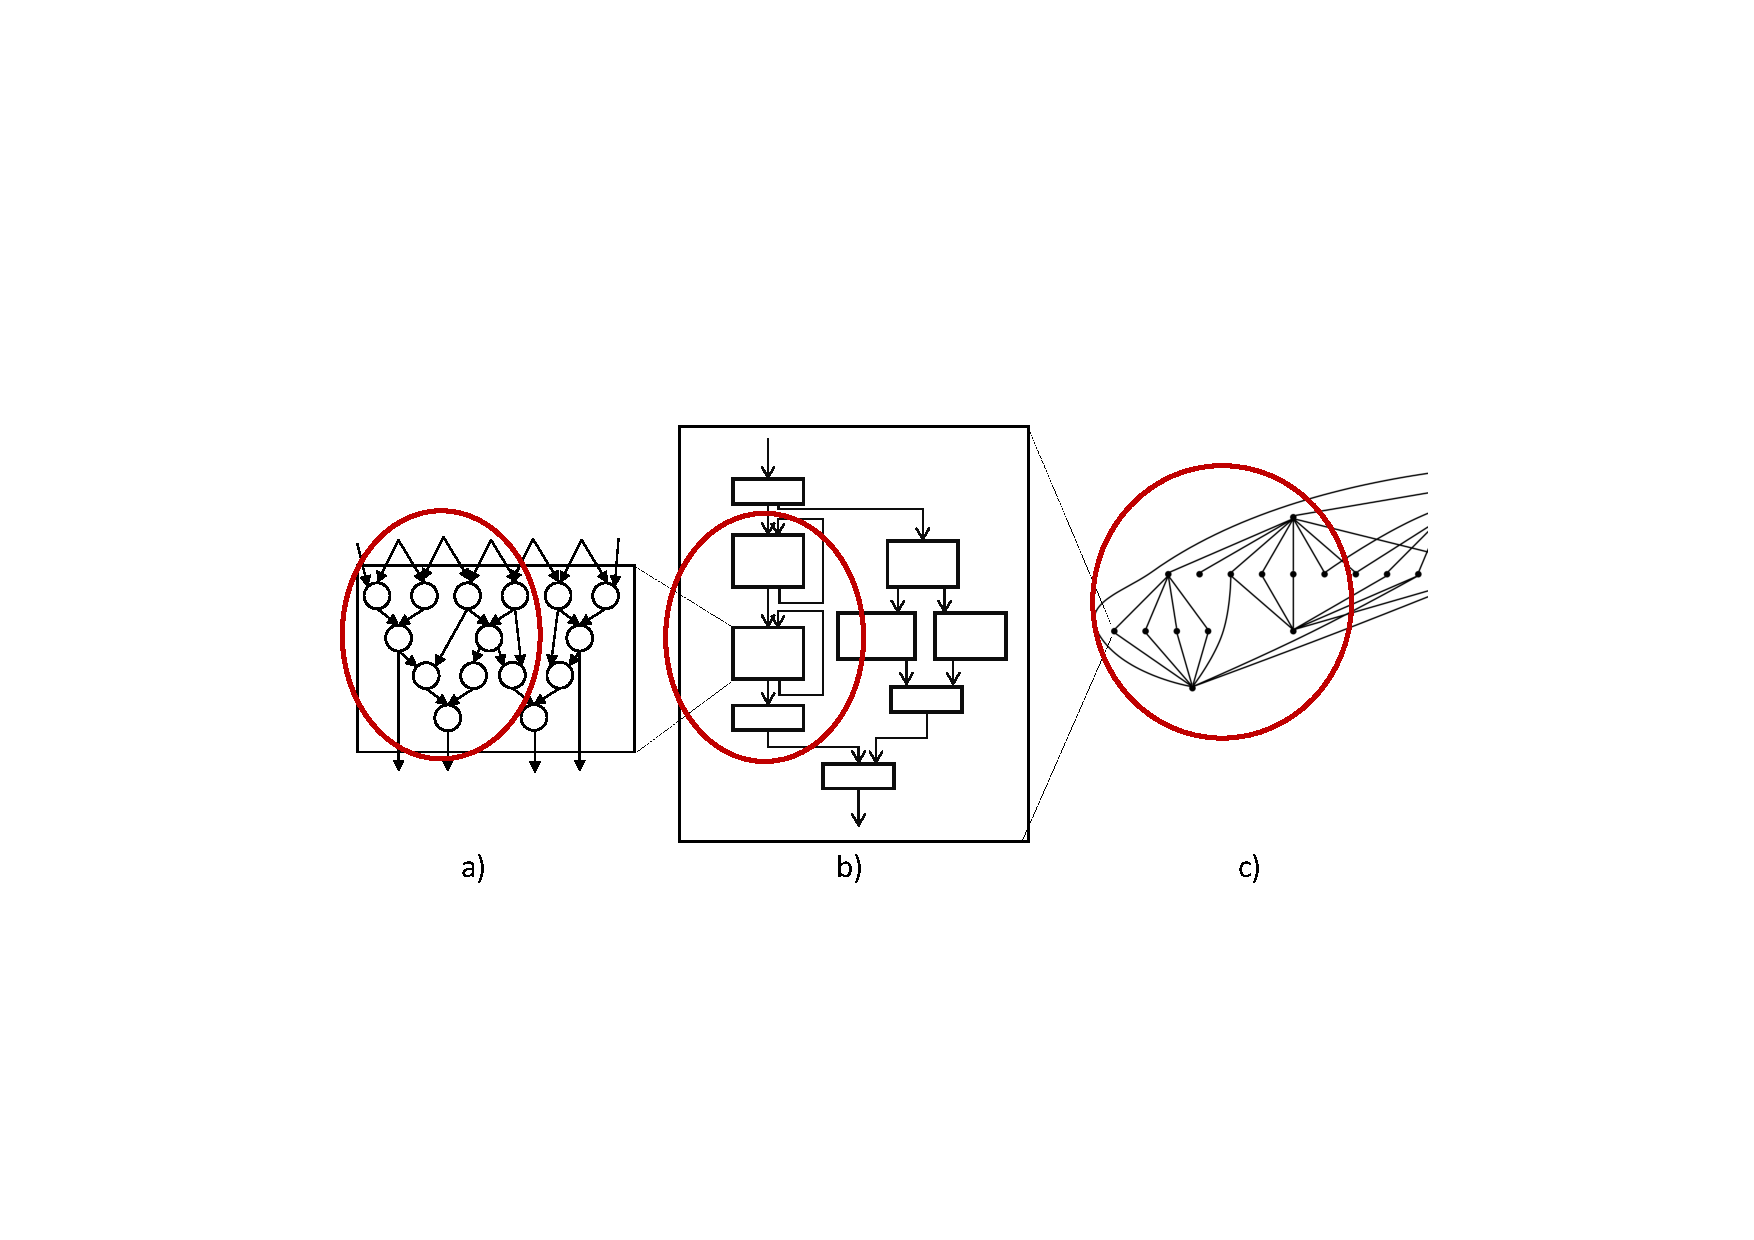
\includegraphics[width= .8 \linewidth]{figs/soa_evolution.pdf}
    \vskip -.5em
  \caption{Evolution of the SoA in automatic selection of custom
          instructions/accelerators: (a) from data-flow level
          \cite{PozziJul06} \cite{GiaquintaMar15}, (b) to control-flow
          level \cite{ZacharopoulosApr19} \cite{OppermannJul16}, (c)
          to function-call graph level (this work).}
  \label{fig:soa-evolution}
  \vskip -1em
\end{figure}

Nonetheless, the automated selection of the application parts most
amenable to HW acceleration is still an open research topic.
Selection approaches based on synthesis results \cite{CanisSep13b}
scale poorly to complex applications, as these are only available late
in the design process.  Estimation frameworks offer a detailed
analysis on the performance and resource requirements of a
HW-accelerated system while avoiding full synthesis runs, either
by interfacing software and HW simulators (e.g., gem5
\cite{BinkertFeb11} and Aladdin \cite{ShaoJul14} in \cite{ShaoOct16}),
or by adopting a hybrid stance, in which HW execution times are
estimated, while software ones are measured on a target platform (as
in Xilinx SdSoC \cite{KathailFeb16}). However, in both cases,
estimations are performed \emph{after} the partitioning of HW
and software, which is left to a trial-and-error basis.  A methodical
solution for partitioning is instead proposed here.\par

The downside of poor partitioning choices, and consequently the
importance of automated tools such \aseeker\ that guide the selection
of high-quality accelerator sets, is even more prominent when
considering the high effort required to optimise the implementation of
HLS-defined accelerators. Design optimisation entails the
specification of multiple directives to steer designs towards the
desired area-performance trade-off. The link between directives and
the performance of implementations is not straightforward, hence
requiring the evaluation of multiple alternatives to reach the
intended results, as exemplified in \cite{SchaferJun12}
\cite{ZuluagaJun12} \cite{FerrettiJan18} \cite{LiuJun13}. It is
therefore key to focus up-front this optimisation effort only on those
candidate accelerators which can lead, from an application
perspective, to tangible speedups.\par

To this end, our approach is inspired by previous works on automatic
identification of instruction set extensions. Most techniques in this
field target customizable processors augmented with
application-specific functional units, within the processor pipelines.
Hence, these techniques usually constrain their search to the scope of
single basic blocks \cite{PozziJul06} \cite{GiaquintaMar15}, as
depicted in Figure~\ref{fig:soa-evolution}a.  Recently, the authors of
\cite{ZacharopoulosApr19} and \cite{OppermannJul16} have instead
targeted the identification of larger code segments, including
control-flow structures belonging to single functions (depicted in
Figure~\ref{fig:soa-evolution}b).  However, such scope still falls
short of the one employed in HLS tools, which are devoted to the
implementation of dedicated accelerators interfaced on a system bus
\cite{CotaJun15}. In this setting, the cost of data movement becomes
so prominent that even control-flow structures inside functions fail
to deliver performance. Suitable accelerator candidates must then
encompass entire functions, including in turn all functions called
within their call tree. \aseeker\ considers this same granularity
(Figure~\ref{fig:soa-evolution}c), advancing the state of the art in
automatic accelerators identification.

\subsection{Methodology}

\subsection{Experimental Results}

\section{EnergySeeker: Accelerators for Energy Efficiency}


\chapter*{Conclusions}
\addcontentsline{toc}{chapter}{Conclusions}


\backmatter

% \chapter{Glossary} %optional

%\bibliographystyle{alpha}
\bibliographystyle{abbrv}
%\bibliographystyle{dcu}
%\bibliographystyle{plainnat}
\bibliography{biblio}

%\bibliographystyle{abbrv}
%note that all bibliography is now in cvs in ../bibl/bibl.bib hence the line below
%\bibliography{/Users/GiorgioZacharo/bibl/bibl}
%
% \cleardoublepage
% \theindex %optional, use only if you have an index, must use
% 	  %\makeindex in the preamble
% \lipsum

\end{document}
